\section{$3$-valent {\sc Eberhard}-like theorems with pentagons}\label{sec:5:3}


In this section we want to prove $3$-valent {\sc Eberhard}-like theorems with pentagons, i.e. for $q = [q_5 \times 5, q_l \times l]$, $w = [w_3 \times 3]$, $l > 6$, $\gcd(q_5, q_l) = 1$. As it turns out in \autoref{sec:negative:results}, this is only possible for all admissible pairs of sequences on all closed orientable $2$-manifolds, if $5 \nmid l$. For all the proofs, we want to use \autoref{thm:main:const}, therefore we need to have a construction scheme for patches with arbitrary large $l$-gons. These we get by the next three constructions:

\begin{construction}\label{const:edge:replacement:5:1}
  \begin{cinput}
  \item A $3$-patch with $p$-vector $p$ and a specified edge with exactly one vertex incident to some $k_1$-gon and the other vertex  incident to some $k_2$-gon.
  \end{cinput}
  \begin{coutput}
  \item A new $3$-patch with $p$-vector $p - [k_1, k_2] + [10k \times 5] + [k_1 + 5k, k_2 + 5k]$ for all $k \in \nats$.
  \item If every two faces of the $3$-patch meet proper, then this is carried over to the new patch.
  \end{coutput}
  \begin{cdescription}
    Using the replacement of the single edge as seen in \autoref{fig:const:edge:replacement:5:1} results in a new map with $p$-vector $p - [k_1, k_2] + [10 \times 5] + [k_1 + 5, k_2 + 5]$. The thick line on the left is the specified edge and the thick line on the right is a new edge which we can use to repeat the construction. Every time we use this construction we add ten new pentagons while increasing the number of vertices of the left and right polygon by 5; doing this $k$ times has the desired result, since we only inserted $3$-valent vertices. That all faces meet proper follows by induction, as this property is preserved in each step.
    \begin{tikzfigure}{\label{fig:const:edge:replacement:5:1}}{}
      \matrix (m) [column sep=1cm] {
        \begin{scope}
          \draw[very thick] (-1, 0) -- (1, 0);
          \draw (-1.2, 0.5) -- (-1, 0) -- (-1.2, -0.5);
          \draw (1.2, 0.5) -- (1, 0) -- (1.2, -0.5);
          \node at (-1.5, 0) {$k_1$};
          \node at (1.5, 0) {$k_2$};
        \end{scope}
        &
        \begin{scope}
          \draw[very thick] (-1, 2.5) -- (1, 2.5);
          \draw (-1, -2.5) -- (1, -2.5);
          \draw (-1.2, 3) -- (-1, 2.5);
          \draw (-1.2, -3) -- (-1, -2.5);
          \draw (1.2, 3) -- (1, 2.5);
          \draw (1.2, -3) -- (1, -2.5);
          \draw (1, 2.5) -- (0.9, 1.5) -- (0.85, 0.5) -- (0.85, -0.5) -- (0.9, -1.5) -- (1, -2.5);
          \draw (-1, 2.5) -- (-0.9, 1.5) -- (-0.85, 0.5) -- (-0.85, -0.5) -- (-0.9, -1.5) -- (-1, -2.5);
          \draw (0.9, 1.5) -- (0, 1.4) -- (-0.9, 1.5);
          \draw (0.9, -1.5) -- (0, -1.4) -- (-0.9, -1.5);
          \draw (0.85, 0.5) -- (0.4, 0.5) -- (0, 0.6) -- (-0.4, 0.5) -- (-0.85, 0.5);
          \draw (0.85, -0.5) -- (0.4, -0.5) -- (0, -0.6) -- (-0.4, -0.5) -- (-0.85, -0.5);
          \draw (0, 1.4) -- (0, 0.6);
          \draw (0, -1.4) -- (0, -0.6);
          \draw (0.4, 0.5) -- (0.3, 0) -- (0.4, -0.5);
          \draw (-0.4, 0.5) -- (-0.3, 0) -- (-0.4, -0.5);
          \draw (0.3, 0) -- (-0.3, 0);
          \node at (-1.8, 0) {$k_1 + 5$};
          \node at (1.8, 0) {$k_2 + 5$};
          \node at (0, 2) {$5$};
          \node at (0, -2) {$5$};
          \node at (0.6, 1) {$5$};
          \node at (-0.6, 1) {$5$};
          \node at (0.6, -1) {$5$};
          \node at (-0.6, -1) {$5$};
          \node at (-0.6, 0) {$5$};
          \node at (0.6, 0) {$5$};
          \node at (0, -0.3) {$5$};
          \node at (0, 0.3) {$5$};
        \end{scope}
        \\
      };
    \end{tikzfigure}
  \end{cdescription}
\end{construction}

\begin{construction}\label{const:edge:replacement:5:2}
  \begin{cinput}
  \item A $3$-patch with $p$-vector $p$ and a specified edge incident to both some $k_1$-gon and some $k_2$-gon.
  \end{cinput}
  \begin{coutput}
  \item A new $3$-patch with $p$-vector $p - [k_1, k_2] + [(10k) \times 5] + [5k + k_1 , 5k + k_2]$ for all $k \in \nats$.
  \end{coutput}
  \begin{cdescription}
    Using the replacement of the single edge as seen in \autoref{fig:const:edge:replacement:5:2} results in a new map with $p$-vector $p - [k_1, k_2] + [10 \times 5] + [k_1 + 5, k_2 + 5]$. The thick line on the left is the specified edge and the thick line on the right is a new edge which we can use to repeat the construction. Every time we use this construction we add four new quadrangles while increasing the number of vertices of the left and right polygon; doing this $k$ times has the desired result, since we only insert $3$-valent vertices.
    \begin{tikzfigure}{\label{fig:const:edge:replacement:5:2}}{}
      \matrix (m) [column sep=1cm] {
        \begin{scope}
          \draw[very thick] (-1, 0) -- (0, 0.2) -- (1, 0);
          \draw (-1.2, 0.5) -- (-1, 0) -- (-1.2, -0.5);
          \draw (1.2, 0.5) -- (1, 0) -- (1.2, -0.5);
          \draw (0, 0.2) -- (0, 0.8);
          \node at (-1.5, 0) {$k_1$};
          \node at (1.5, 0) {$k_2$};
        \end{scope}
        &
        \begin{scope}
          \draw (0, 2.7) -- (0, 3.3);
          \draw[very thick] (1, 2.5) -- (0, 2.7) -- (-1, 2.5);
          \draw (-0.9, 1.5) -- (0.9, 1.5);
          \draw (-1.2, 3) -- (-1, 2.5);
          \draw (-1.2, -3) -- (-1, -2.5);
          \draw (1.2, 3) -- (1, 2.5);
          \draw (1.2, -3) -- (1, -2.5);
          \draw (1, 2.5) -- (0.9, 1.5) -- (0.85, 0.5) -- (0.85, -0.5) -- (0.9, -1.5) -- (1, -2.5);
          \draw (-1, 2.5) -- (-0.9, 1.5) -- (-0.85, 0.5) -- (-0.85, -0.5) -- (-0.9, -1.5) -- (-1, -2.5);
          \draw (0.85, 0.5) -- (0, 0.4) -- (-0.85, 0.5);
          \draw (-1, -2.5) -- (0, -2.3) -- (1, -2.5);
          \draw (0.85, -0.5) -- (0.4, -0.5) -- (0, -0.4) -- (-0.4, -0.5) -- (-0.85, -0.5);
          \draw (0.9, -1.5) -- (0.4, -1.5) -- (0, -1.6) -- (-0.4, -1.5) -- (-0.9, -1.5);
          \draw (0, 0.4) -- (0, -0.4);
          \draw (0, -2.3) -- (0, -1.6);
          \draw (0.4, -0.5) -- (0.3, -1) -- (0.4, -1.5);
          \draw (-0.4, -0.5) -- (-0.3, -1) -- (-0.4, -1.5);
          \draw (0.3, -1) -- (-0.3, -1);
          \node at (-1.8, 0) {$k_1 + 5$};
          \node at (1.8, 0) {$k_2 + 5$};
          \node at (0, 1) {$5$};
          \node at (0, 2) {$5$};
          \node at (0.6, 0) {$5$};
          \node at (-0.6, 0) {$5$};
          \node at (0.6, -2) {$5$};
          \node at (-0.6, -2) {$5$};
          \node at (-0.6, -1) {$5$};
          \node at (0.6, -1) {$5$};
          \node at (0, -1.3) {$5$};
          \node at (0, -0.7) {$5$};
        \end{scope}
        \\
      };
    \end{tikzfigure}
  \end{cdescription}
\end{construction}

\begin{construction}\label{const:edge:replacement:5:3}
  \begin{cinput}
  \item A $3$-patch with $p$-vector $p$ and a specified edge incident to both some $k_1$-gon and some $k_2$-gon.
  \end{cinput}
  \begin{coutput}
  \item A new $3$-patch with $p$-vector $p - [k_1, k_2] + [(10k) \times 5] + [5k + k_1 , 5k + k_2]$ for all $k \in \nats$.
  \end{coutput}
  \begin{cdescription}
    Using the replacement of the single edge as seen in \autoref{fig:const:edge:replacement:5:3} results in a new map with $p$-vector $p - [k_1, k_2] + [10 \times 5] + [k_1 + 5, k_2 + 5]$. The thick line on the left is the specified edge and the thick line on the right is a new edge which we can use to repeat the construction. Every time we use this construction we add four new quadrangles while increasing the number of vertices of the left and right polygon; doing this $k$ times has the desired result, since we only insert $3$-valent vertices.
    \begin{tikzfigure}{\label{fig:const:edge:replacement:5:3}}{}
      \matrix (m) [column sep=1cm] {
        \begin{scope}
          \draw[very thick] (0, -1) -- (0, 1);
          \draw (0.5, -1.2) -- (0, -1) -- (-0.5, -1.2);
          \draw (0.5, 1.2) -- (0, 1) -- (-0.5, 1.2);
          \node at (-1, 0) {$k_1$};
          \node at (1, 0) {$k_2$};
        \end{scope}
        &
        \begin{scope}
          \draw (0.5, -2.7) -- (0, -2.5) -- (-0.5, -2.7);
          \draw (0.5, 2.7) -- (0, 2.5) -- (-0.5, 2.7);
          \draw[very thick] (0, 2.5) -- (0, 2);
          \draw (0, -2.5) -- (0, -2);
          \draw (0, -2) -- (-1.5 , -1.5) -- (-2, 0) -- (-1.5, 1.5) -- (0, 2) -- (1.5, 1.5) -- (2, 0) -- (1.5, -1.5) -- (0, -2);
          \draw (-0.5, -1) -- (-0.5, -0.5) -- (-1, 0) -- (-0.5, 0.5) -- (-0.5, 1) -- (0.5, 1) -- (0.5, 0.5) -- (1, 0) -- (0.5, -0.5) -- (0.5, -1) -- (-0.5, -1);
          \draw (-0.5, -0.5) -- (0, -0.25) -- (0.5, -0.5);
          \draw (-0.5, 0.5) -- (0, 0.25) -- (0.5, 0.5);
          \draw (-1.5, -1.5) -- (-0.5, -1);
          \draw (1.5, -1.5) -- (0.5, -1);
          \draw (-1.5, 1.5) -- (-0.5, 1);
          \draw (1.5, 1.5) -- (0.5, 1);
          \draw (0, -0.25) -- (0, 0.25);
          \draw (-2, 0) -- (-1, 0);
          \draw (2, 0) -- (1, 0);

          \node at (-1.25, -0.5) {$5$};
          \node at (1.25, -0.5) {$5$};
          \node at (-1.25, 0.5) {$5$};
          \node at (1.25, 0.5) {$5$};
          \node at (-0.5, 0) {$5$};
          \node at (0.5, 0) {$5$};
          \node at (0, -1.5) {$5$};
          \node at (0, 1.5) {$5$};
          \node at (0, -0.75) {$5$};
          \node at (0, 0.75) {$5$};
          \node[anchor=east] at (-2, 0) {$k_1 + 5$};
          \node[anchor=west] at (2, 0) {$k_2 + 5$};
        \end{scope}
        \\
      };
    \end{tikzfigure}
  \end{cdescription}
\end{construction}


We now can split the infinitely many cases in four series, each with a different residual class of $l \mod 5$:

\begin{theorem}
  Let $p$ and $v$ be a pair of admissible sequences for a orientable closed $2$-manifold $S$. Then $(p, v)$ is $[(5k + 1) \times 5, (5k+7)]$-$[3]$-realizable for all $k \in \nats$.
  \begin{proof}
    An expansion $3$-patch with outer tuple $o = (1, 1, 1, 2, 2, 2)$, a corresponding $o$-$6$-gonal $3$-patch and a expansion $3$-patch with the polyhedral property, all consisting only of pentagons and heptagons, are shown in \autoref{fig:expansion:patch:5:7}. Using \autoref{const:edge:replacement:5:1}, \autoref{const:edge:replacement:5:2} and \autoref{const:edge:replacement:5:3} on the edges as indicated in all three we get new $3$-patches consisting only of pentagons and $5k + 7$-gons. Therefore we can apply \autoref{thm:main:const}.
    \begin{tikzfigure}{\label{fig:expansion:patch:5:7}}{}
      \matrix (m) [column sep=1cm, row sep=1cm] {
        \begin{scope}[yscale=0.866]
          \draw[very thick] (-0.5, 1) -- (-2.5, 5) -- (-4.5, 6.333) -- (-4, 8) -- (-4.5, 9) -- (-4, 10) -- (-2.5, 10.333) -- (-1, 10) -- (-0.5, 9) -- (0.5, 9) -- (1, 8) -- (2.5, 7.666) -- (2.5, 5) -- (0.5, 1) -- (-0.5, 1);
          \draw (-2.5, 5) -- (-2, 6) -- (1, 8);
          \draw (-2, 6) -- (-2, 8) -- (-4, 8);
          \draw (-2, 8) -- (-0.5, 9);
        \end{scope}
        &
        \begin{scope}[scale=0.5]
          % \coordinate (x0) at (0.600709, 0.137377);
\coordinate (x1) at (0.770222, -0.102367);
\coordinate (x2) at (0.939693, -0.342020);
\coordinate (x3) at (0.939693, 0.342020);
\coordinate (x4) at (0.196651, 0.069275);
\coordinate (x5) at (0.500000, -0.866025);
\coordinate (x6) at (0.500000, 0.866025);
\coordinate (x7) at (-0.173648, 0.984808);
\coordinate (x8) at (-0.766044, 0.642788);
\coordinate (x9) at (-1.000000, 0.000000);
\coordinate (x10) at (-0.766044, -0.642788);
\coordinate (x11) at (-0.173648, -0.984808);
\draw (0.600709, 0.137377) -- (0.770222, -0.102367);
\draw (0.770222, -0.102367) -- (0.939693, -0.342020);
\draw (0.939693, -0.342020) -- (0.939693, 0.342020);
\draw (0.939693, 0.342020) -- (0.600709, 0.137377);
\draw (0.600709, 0.137377) -- (0.196651, 0.069275);
\draw (0.196651, 0.069275) -- (0.500000, -0.866025);
\draw (0.500000, -0.866025) -- (0.939693, -0.342020);
\draw (0.939693, 0.342020) -- (0.500000, 0.866025);
\draw (0.500000, 0.866025) -- (-0.173648, 0.984808);
\draw (-0.173648, 0.984808) -- (0.196651, 0.069275);
\draw (-0.173648, 0.984808) -- (-0.766044, 0.642788);
\draw (-0.766044, 0.642788) -- (-1.000000, 0.000000);
\draw (-1.000000, 0.000000) -- (-0.766044, -0.642788);
\draw (-0.766044, -0.642788) -- (-0.173648, -0.984808);
\draw (-0.173648, -0.984808) -- (0.500000, -0.866025);

          \begin{scope}[yscale=0.866]
            \draw[very thick] (-0.5, 1) -- (-2.5, 5) -- (-4.5, 6.333) -- (-4, 8) -- (-4.5, 9) -- (-4, 10) -- (-2.5, 10.333) -- (-1, 10) -- (-0.5, 9) -- (0.5, 9) -- (1, 8) -- (2.5, 7.666) -- (2.5, 5) -- (0.5, 1) -- (-0.5, 1);
            \draw (-2.5, 5) -- (-2, 6) -- (1, 8);
            \draw (-2, 6) -- (-2, 8) -- (-4, 8);
            \draw (-2, 8) -- (-0.5, 9);
          \end{scope}
          \begin{scope}[rotate=-60, yscale=0.866]
            \draw[very thick] (-0.5, 1) -- (-2.5, 5) -- (-4.5, 6.333) -- (-4, 8) -- (-4.5, 9) -- (-4, 10) -- (-2.5, 10.333) -- (-1, 10) -- (-0.5, 9) -- (0.5, 9) -- (1, 8) -- (2.5, 7.666) -- (2.5, 5) -- (0.5, 1) -- (-0.5, 1);
            \draw (-2.5, 5) -- (-2, 6) -- (1, 8);
            \draw (-2, 6) -- (-2, 8) -- (-4, 8);
            \draw (-2, 8) -- (-0.5, 9);
          \end{scope}
          \begin{scope}[yscale=0.866,shift={(0 cm,18 cm)},rotate=180]
            \draw[very thick] (-0.5, 1) -- (-2.5, 5) -- (-4.5, 6.333) -- (-4, 8) -- (-4.5, 9) -- (-4, 10) -- (-2.5, 10.333) -- (-1, 10) -- (-0.5, 9) -- (0.5, 9) -- (1, 8) -- (2.5, 7.666) -- (2.5, 5) -- (0.5, 1) -- (-0.5, 1);
            \draw (-2.5, 5) -- (-2, 6) -- (1, 8);
            \draw (-2, 6) -- (-2, 8) -- (-4, 8);
            \draw (-2, 8) -- (-0.5, 9);
          \end{scope}
          \begin{scope}[shift={(0 cm,15.588 cm)},rotate=120,yscale=0.866]
            \draw[very thick] (-0.5, 1) -- (-2.5, 5) -- (-4.5, 6.333) -- (-4, 8) -- (-4.5, 9) -- (-4, 10) -- (-2.5, 10.333) -- (-1, 10) -- (-0.5, 9) -- (0.5, 9) -- (1, 8) -- (2.5, 7.666) -- (2.5, 5) -- (0.5, 1) -- (-0.5, 1);
            \draw (-2.5, 5) -- (-2, 6) -- (1, 8);
            \draw (-2, 6) -- (-2, 8) -- (-4, 8);
            \draw (-2, 8) -- (-0.5, 9);
          \end{scope}
        \end{scope}
        \\
        \begin{scope}[scale=3, yshift=25]
          \coordinate (x0) at (-0.882596, 0.144489);
\coordinate (x1) at (-0.817805, 0.052066);
\coordinate (x2) at (-0.717351, 0.117014);
\coordinate (x3) at (-0.680700, 0.275346);
\coordinate (x4) at (-0.812941, 0.277494);
\coordinate (x5) at (-0.998308, 0.058145);
\coordinate (x6) at (-0.998308, -0.058145);
\coordinate (x7) at (-0.854325, -0.072140);
\coordinate (x8) at (-0.746725, -0.176568);
\coordinate (x9) at (-0.695612, -0.029457);
\coordinate (x10) at (-0.577701, -0.003240);
\coordinate (x11) at (-0.572673, 0.412353);
\coordinate (x12) at (-0.847214, 0.420134);
\coordinate (x13) at (-0.984808, 0.173648);
\coordinate (x14) at (-0.711199, -0.354740);
\coordinate (x15) at (-0.572753, -0.418177);
\coordinate (x16) at (-0.549509, 0.835488);
\coordinate (x17) at (-0.642788, 0.766044);
\coordinate (x18) at (-0.727374, 0.686242);
\coordinate (x19) at (-0.984808, -0.173648);
\coordinate (x20) at (-0.957990, -0.286803);
\coordinate (x21) at (-0.782466, -0.508334);
\coordinate (x22) at (-0.642788, -0.766044);
\coordinate (x23) at (-0.549509, -0.835488);
\coordinate (x24) at (-0.448799, -0.893633);
\coordinate (x25) at (-0.448799, 0.893633);
\coordinate (x26) at (-0.342020, -0.939693);
\coordinate (x27) at (-0.230616, -0.973045);
\coordinate (x28) at (0.022529, -0.386804);
\coordinate (x29) at (-0.022528, 0.386799);
\coordinate (x30) at (-0.342020, 0.939693);
\coordinate (x31) at (0.342020, -0.939693);
\coordinate (x32) at (0.448799, -0.893633);
\coordinate (x33) at (0.448799, 0.893633);
\coordinate (x34) at (0.342020, 0.939693);
\coordinate (x35) at (0.230616, 0.973045);
\coordinate (x36) at (0.549509, -0.835488);
\coordinate (x37) at (0.648552, -0.425935);
\coordinate (x38) at (0.716422, -0.012589);
\coordinate (x39) at (0.655278, 0.408542);
\coordinate (x40) at (0.549509, 0.835488);
\coordinate (x41) at (0.826848, -0.421223);
\coordinate (x42) at (0.984808, -0.173648);
\coordinate (x43) at (0.998308, -0.058145);
\coordinate (x44) at (0.998308, 0.058145);
\coordinate (x45) at (0.841254, 0.282416);
\coordinate (x46) at (0.792667, 0.497122);
\coordinate (x47) at (0.642788, 0.766044);
\coordinate (x48) at (0.642788, -0.766044);
\coordinate (x49) at (0.727374, -0.686242);
\coordinate (x50) at (0.984808, 0.173648);
\coordinate (x51) at (0.957990, 0.286803);
\coordinate (x52) at (0.918216, 0.396080);
\coordinate (x53) at (0.866025, 0.500000);
\coordinate (x54) at (0.802123, 0.597159);
\coordinate (x55) at (0.727374, 0.686242);
\coordinate (x56) at (0.116093, 0.993238);
\coordinate (x57) at (0.000000, 1.000000);
\coordinate (x58) at (-0.116093, 0.993238);
\coordinate (x59) at (-0.230616, 0.973045);
\coordinate (x60) at (-0.802123, 0.597159);
\coordinate (x61) at (-0.866025, 0.500000);
\coordinate (x62) at (-0.918216, 0.396080);
\coordinate (x63) at (-0.957990, 0.286803);
\coordinate (x64) at (-0.918216, -0.396080);
\coordinate (x65) at (-0.866025, -0.500000);
\coordinate (x66) at (-0.802123, -0.597159);
\coordinate (x67) at (-0.727374, -0.686242);
\coordinate (x68) at (-0.116093, -0.993238);
\coordinate (x69) at (-0.000000, -1.000000);
\coordinate (x70) at (0.116093, -0.993238);
\coordinate (x71) at (0.230616, -0.973045);
\coordinate (x72) at (0.802123, -0.597159);
\coordinate (x73) at (0.866025, -0.500000);
\coordinate (x74) at (0.918216, -0.396080);
\coordinate (x75) at (0.957990, -0.286803);

\draw (-0.882596, 0.144489) -- (-0.817805, 0.052066);
\draw (-0.817805, 0.052066) -- (-0.717351, 0.117014);
\draw (-0.717351, 0.117014) -- (-0.680700, 0.275346);
\draw (-0.680700, 0.275346) -- (-0.812941, 0.277494);
\draw (-0.812941, 0.277494) -- (-0.882596, 0.144489);
\draw (-0.882596, 0.144489) -- (-0.998308, 0.058145);
\draw (-0.998308, 0.058145) -- (-0.998308, -0.058145);
\draw (-0.998308, -0.058145) -- (-0.854325, -0.072140);
\draw (-0.854325, -0.072140) -- (-0.817805, 0.052066);
\draw (-0.854325, -0.072140) -- (-0.746725, -0.176568);
\draw (-0.746725, -0.176568) -- (-0.695612, -0.029457);
\draw (-0.695612, -0.029457) -- (-0.717351, 0.117014);
\draw (-0.695612, -0.029457) -- (-0.577701, -0.003240);
\draw (-0.577701, -0.003240) -- (-0.572673, 0.412353);
\draw (-0.572673, 0.412353) -- (-0.680700, 0.275346);
\draw (-0.812941, 0.277494) -- (-0.847214, 0.420134);
\draw (-0.847214, 0.420134) -- (-0.984808, 0.173648);
\draw (-0.984808, 0.173648) -- (-0.998308, 0.058145);
\draw (-0.746725, -0.176568) -- (-0.711199, -0.354740);
\draw (-0.711199, -0.354740) -- (-0.572753, -0.418177);
\draw (-0.572753, -0.418177) -- (-0.577701, -0.003240);
\draw (-0.572673, 0.412353) -- (-0.549509, 0.835488);
\draw (-0.549509, 0.835488) -- (-0.642788, 0.766044);
\draw (-0.642788, 0.766044) -- (-0.727374, 0.686242);
\draw[ldiamond] (-0.727374, 0.686242) -- (-0.847214, 0.420134);
\draw (-0.998308, -0.058145) -- (-0.984808, -0.173648);
\draw (-0.984808, -0.173648) -- (-0.957990, -0.286803);
\draw[ldiamond] (-0.957990, -0.286803) -- (-0.782466, -0.508334);
\draw (-0.782466, -0.508334) -- (-0.711199, -0.354740);
\draw (-0.782466, -0.508334) -- (-0.642788, -0.766044);
\draw (-0.642788, -0.766044) -- (-0.549509, -0.835488);
\draw (-0.549509, -0.835488) -- (-0.572753, -0.418177);
\draw (-0.549509, -0.835488) -- (-0.448799, -0.893633);
\draw[ldiamond] (-0.448799, -0.893633) -- (-0.448799, 0.893633);
\draw (-0.448799, 0.893633) -- (-0.549509, 0.835488);
\draw (-0.448799, -0.893633) -- (-0.342020, -0.939693);
\draw (-0.342020, -0.939693) -- (-0.230616, -0.973045);
\draw (-0.230616, -0.973045) -- (0.022529, -0.386804);
\draw[very thick] (0.022529, -0.386804) -- (-0.022528, 0.386799);
\draw (-0.022528, 0.386799) -- (-0.342020, 0.939693);
\draw (-0.342020, 0.939693) -- (-0.448799, 0.893633);
\draw (0.022529, -0.386804) -- (0.342020, -0.939693);
\draw (0.342020, -0.939693) -- (0.448799, -0.893633);
\draw (0.448799, -0.893633) -- (0.448799, 0.893633);
\draw (0.448799, 0.893633) -- (0.342020, 0.939693);
\draw (0.342020, 0.939693) -- (0.230616, 0.973045);
\draw (0.230616, 0.973045) -- (-0.022528, 0.386799);
\draw (0.448799, -0.893633) -- (0.549509, -0.835488);
\draw (0.549509, -0.835488) -- (0.648552, -0.425935);
\draw (0.648552, -0.425935) -- (0.716422, -0.012589);
\draw (0.716422, -0.012589) -- (0.655278, 0.408542);
\draw (0.655278, 0.408542) -- (0.549509, 0.835488);
\draw[very thick] (0.549509, 0.835488) -- (0.448799, 0.893633);
\draw (0.648552, -0.425935) -- (0.826848, -0.421223);
\draw (0.826848, -0.421223) -- (0.984808, -0.173648);
\draw (0.984808, -0.173648) -- (0.998308, -0.058145);
\draw (0.998308, -0.058145) -- (0.716422, -0.012589);
\draw (0.998308, -0.058145) -- (0.998308, 0.058145);
\draw (0.998308, 0.058145) -- (0.841254, 0.282416);
\draw (0.841254, 0.282416) -- (0.655278, 0.408542);
\draw (0.841254, 0.282416) -- (0.792667, 0.497122);
\draw (0.792667, 0.497122) -- (0.642788, 0.766044);
\draw[very thick] (0.642788, 0.766044) -- (0.549509, 0.835488);
\draw[very thick] (0.549509, -0.835488) -- (0.642788, -0.766044);
\draw[very thick] (0.642788, -0.766044) -- (0.727374, -0.686242);
\draw (0.727374, -0.686242) -- (0.826848, -0.421223);
\draw (0.998308, 0.058145) -- (0.984808, 0.173648);
\draw (0.984808, 0.173648) -- (0.957990, 0.286803);
\draw (0.957990, 0.286803) -- (0.792667, 0.497122);
\draw (0.957990, 0.286803) -- (0.918216, 0.396080);
\draw (0.918216, 0.396080) -- (0.866025, 0.500000);
\draw (0.866025, 0.500000) -- (0.802123, 0.597159);
\draw (0.802123, 0.597159) -- (0.727374, 0.686242);
\draw (0.727374, 0.686242) -- (0.642788, 0.766044);
\draw (0.230616, 0.973045) -- (0.116093, 0.993238);
\draw (0.116093, 0.993238) -- (0.000000, 1.000000);
\draw (0.000000, 1.000000) -- (-0.116093, 0.993238);
\draw (-0.116093, 0.993238) -- (-0.230616, 0.973045);
\draw (-0.230616, 0.973045) -- (-0.342020, 0.939693);
\draw (-0.727374, 0.686242) -- (-0.802123, 0.597159);
\draw (-0.802123, 0.597159) -- (-0.866025, 0.500000);
\draw (-0.866025, 0.500000) -- (-0.918216, 0.396080);
\draw (-0.918216, 0.396080) -- (-0.957990, 0.286803);
\draw (-0.957990, 0.286803) -- (-0.984808, 0.173648);
\draw (-0.957990, -0.286803) -- (-0.918216, -0.396080);
\draw (-0.918216, -0.396080) -- (-0.866025, -0.500000);
\draw (-0.866025, -0.500000) -- (-0.802123, -0.597159);
\draw (-0.802123, -0.597159) -- (-0.727374, -0.686242);
\draw (-0.727374, -0.686242) -- (-0.642788, -0.766044);
\draw (-0.230616, -0.973045) -- (-0.116093, -0.993238);
\draw (-0.116093, -0.993238) -- (-0.000000, -1.000000);
\draw (-0.000000, -1.000000) -- (0.116093, -0.993238);
\draw (0.116093, -0.993238) -- (0.230616, -0.973045);
\draw (0.230616, -0.973045) -- (0.342020, -0.939693);
\draw (0.727374, -0.686242) -- (0.802123, -0.597159);
\draw (0.802123, -0.597159) -- (0.866025, -0.500000);
\draw (0.866025, -0.500000) -- (0.918216, -0.396080);
\draw (0.918216, -0.396080) -- (0.957990, -0.286803);
\draw (0.957990, -0.286803) -- (0.984808, -0.173648);

\fill[black] (-0.882596, 0.144489) circle (0.2pt);
\fill[black] (-0.817805, 0.052066) circle (0.2pt);
\fill[black] (-0.717351, 0.117014) circle (0.2pt);
\fill[black] (-0.680700, 0.275346) circle (0.2pt);
\fill[black] (-0.812941, 0.277494) circle (0.2pt);
\fill[black] (-0.998308, 0.058145) circle (0.2pt);
\fill[black] (-0.998308, -0.058145) circle (0.2pt);
\fill[black] (-0.854325, -0.072140) circle (0.2pt);
\fill[black] (-0.746725, -0.176568) circle (0.2pt);
\fill[black] (-0.695612, -0.029457) circle (0.2pt);
\fill[black] (-0.577701, -0.003240) circle (0.2pt);
\fill[black] (-0.572673, 0.412353) circle (0.2pt);
\fill[black] (-0.847214, 0.420134) circle (0.2pt);
\fill[black] (-0.984808, 0.173648) circle (0.2pt);
\fill[black] (-0.711199, -0.354740) circle (0.2pt);
\fill[black] (-0.572753, -0.418177) circle (0.2pt);
\fill[black] (-0.549509, 0.835488) circle (0.2pt);
\fill[black] (-0.642788, 0.766044) circle (0.2pt);
\fill[black] (-0.727374, 0.686242) circle (0.2pt);
\fill[black] (-0.984808, -0.173648) circle (0.2pt);
\fill[black] (-0.957990, -0.286803) circle (0.2pt);
\fill[black] (-0.782466, -0.508334) circle (0.2pt);
\fill[black] (-0.642788, -0.766044) circle (0.2pt);
\fill[black] (-0.549509, -0.835488) circle (0.2pt);
\fill[black] (-0.448799, -0.893633) circle (0.2pt);
\fill[black] (-0.448799, 0.893633) circle (0.2pt);
\fill[black] (-0.342020, -0.939693) circle (0.2pt);
\fill[black] (-0.230616, -0.973045) circle (0.2pt);
\fill[black] (0.022529, -0.386804) circle (0.2pt);
\fill[black] (-0.022528, 0.386799) circle (0.2pt);
\fill[black] (-0.342020, 0.939693) circle (0.2pt);
\fill[black] (0.342020, -0.939693) circle (0.2pt);
\fill[black] (0.448799, -0.893633) circle (0.2pt);
\fill[black] (0.448799, 0.893633) circle (0.2pt);
\fill[black] (0.342020, 0.939693) circle (0.2pt);
\fill[black] (0.230616, 0.973045) circle (0.2pt);
\fill[black] (0.549509, -0.835488) circle (0.2pt);
\fill[black] (0.648552, -0.425935) circle (0.2pt);
\fill[black] (0.716422, -0.012589) circle (0.2pt);
\fill[black] (0.655278, 0.408542) circle (0.2pt);
\fill[black] (0.549509, 0.835488) circle (0.2pt);
\fill[black] (0.826848, -0.421223) circle (0.2pt);
\fill[black] (0.984808, -0.173648) circle (0.2pt);
\fill[black] (0.998308, -0.058145) circle (0.2pt);
\fill[black] (0.998308, 0.058145) circle (0.2pt);
\fill[black] (0.841254, 0.282416) circle (0.2pt);
\fill[black] (0.792667, 0.497122) circle (0.2pt);
\fill[black] (0.642788, 0.766044) circle (0.2pt);
\fill[black] (0.642788, -0.766044) circle (0.2pt);
\fill[black] (0.727374, -0.686242) circle (0.2pt);
\fill[black] (0.984808, 0.173648) circle (0.2pt);
\fill[black] (0.957990, 0.286803) circle (0.2pt);
\fill[black] (0.918216, 0.396080) circle (0.2pt);
\fill[black] (0.866025, 0.500000) circle (0.2pt);
\fill[black] (0.802123, 0.597159) circle (0.2pt);
\fill[black] (0.727374, 0.686242) circle (0.2pt);
\fill[black] (0.116093, 0.993238) circle (0.2pt);
\fill[black] (0.000000, 1.000000) circle (0.2pt);
\fill[black] (-0.116093, 0.993238) circle (0.2pt);
\fill[black] (-0.230616, 0.973045) circle (0.2pt);
\fill[black] (-0.802123, 0.597159) circle (0.2pt);
\fill[black] (-0.866025, 0.500000) circle (0.2pt);
\fill[black] (-0.918216, 0.396080) circle (0.2pt);
\fill[black] (-0.957990, 0.286803) circle (0.2pt);
\fill[black] (-0.918216, -0.396080) circle (0.2pt);
\fill[black] (-0.866025, -0.500000) circle (0.2pt);
\fill[black] (-0.802123, -0.597159) circle (0.2pt);
\fill[black] (-0.727374, -0.686242) circle (0.2pt);
\fill[black] (-0.116093, -0.993238) circle (0.2pt);
\fill[black] (-0.000000, -1.000000) circle (0.2pt);
\fill[black] (0.116093, -0.993238) circle (0.2pt);
\fill[black] (0.230616, -0.973045) circle (0.2pt);
\fill[black] (0.802123, -0.597159) circle (0.2pt);
\fill[black] (0.866025, -0.500000) circle (0.2pt);
\fill[black] (0.918216, -0.396080) circle (0.2pt);
\fill[black] (0.957990, -0.286803) circle (0.2pt);

        \end{scope}
        \\
      };
    \end{tikzfigure}
  \end{proof}
\end{theorem}

\begin{theorem}
  Let $p$ and $v$ be a pair of admissible sequences for a orientable closed $2$-manifold $S$. Then $(p, v)$ is $[(5k + 2) \times 5, (5k+8)]$-$[3]$-realizable for all $k \in \nats$.
  \begin{proof}
    An expansion $3$-patch with outer tuple $o = (1, 2, 2, 2, 1, 2, 1, 1, 1, 2)$, a corresponding $o$-$6$-gonal $3$-patch and a expansion $3$-patch with the polyhedral property, all consisting only of pentagons and octagons, are shown in \autoref{fig:expansion:patch:5:8}. Using \autoref{const:edge:replacement:5:1}, \autoref{const:edge:replacement:5:2} and \autoref{const:edge:replacement:5:3} on the edges as indicated in all three we get new $3$-patches consisting only of pentagons and $5k + 8$-gons. Therefore we can apply \autoref{thm:main:const}.
    \begin{tikzfigure}{\label{fig:expansion:patch:5:8}}{}
      \matrix (m) [column sep=1cm] {
        \begin{scope}[scale=0.5]
          \begin{scope}[yscale=0.866]
            \draw[very thick] (-0.5, 1) -- (0.5, 5) -- (-0.5, 9) -- (-1.5, 11);
            % \coordinate (x0) at (0.568199, -0.201929);
\coordinate (x1) at (0.448960, -0.399099);
\coordinate (x2) at (0.328743, -0.595831);
\coordinate (x3) at (0.654861, -0.755750);
\coordinate (x4) at (0.959493, -0.281733);
\coordinate (x5) at (0.204800, -0.052065);
\coordinate (x6) at (-0.032816, -0.518344);
\coordinate (x7) at (-0.415415, -0.909632);
\coordinate (x8) at (0.142315, -0.989821);
\coordinate (x9) at (0.959493, 0.281733);
\coordinate (x10) at (0.236438, 0.479720);
\coordinate (x11) at (-0.415415, 0.909632);
\coordinate (x12) at (-0.841254, 0.540641);
\coordinate (x13) at (-1.000000, 0.000000);
\coordinate (x14) at (-0.841254, -0.540641);
\coordinate (x15) at (0.654861, 0.755750);
\coordinate (x16) at (0.142315, 0.989821);
\draw (0.568199, -0.201929) -- (0.448960, -0.399099);
\draw (0.448960, -0.399099) -- (0.328743, -0.595831);
\draw (0.328743, -0.595831) -- (0.654861, -0.755750);
\draw (0.654861, -0.755750) -- (0.959493, -0.281733);
\draw (0.959493, -0.281733) -- (0.568199, -0.201929);
\draw (0.568199, -0.201929) -- (0.204800, -0.052065);
\draw (0.204800, -0.052065) -- (-0.032816, -0.518344);
\draw (-0.032816, -0.518344) -- (0.328743, -0.595831);
\draw (-0.032816, -0.518344) -- (-0.415415, -0.909632);
\draw (-0.415415, -0.909632) -- (0.142315, -0.989821);
\draw (0.142315, -0.989821) -- (0.654861, -0.755750);
\draw (0.959493, -0.281733) -- (0.959493, 0.281733);
\draw (0.959493, 0.281733) -- (0.236438, 0.479720);
\draw (0.236438, 0.479720) -- (0.204800, -0.052065);
\draw (0.236438, 0.479720) -- (-0.415415, 0.909632);
\draw (-0.415415, 0.909632) -- (-0.841254, 0.540641);
\draw (-0.841254, 0.540641) -- (-1.000000, 0.000000);
\draw (-1.000000, 0.000000) -- (-0.841254, -0.540641);
\draw (-0.841254, -0.540641) -- (-0.415415, -0.909632);
\draw (0.959493, 0.281733) -- (0.654861, 0.755750);
\draw (0.654861, 0.755750) -- (0.142315, 0.989821);
\draw (0.142315, 0.989821) -- (-0.415415, 0.909632);
\node at (-0.000000, -0.000000) {0};
\node at (0.592051, -0.446868) {1};
\node at (0.303577, -0.353454) {2};
\node at (0.135537, -0.753876) {3};
\node at (0.585685, 0.045145) {4};
\node at (-0.388114, -0.011336) {5};
\node at (0.315538, 0.683331) {6};

          \end{scope}
        \end{scope}
        \\
        \begin{scope}[scale=3, yshift=25]
          \coordinate (x0) at (-0.297003, 0.445473);
\coordinate (x1) at (-0.470182, 0.606872);
\coordinate (x2) at (-0.630409, 0.404927);
\coordinate (x3) at (-0.747357, 0.175386);
\coordinate (x4) at (-0.528641, 0.085018);
\coordinate (x5) at (-0.009460, 0.760053);
\coordinate (x6) at (-0.371662, 0.928368);
\coordinate (x7) at (-0.458227, 0.888835);
\coordinate (x8) at (-0.540641, 0.841254);
\coordinate (x9) at (-0.756908, 0.486478);
\coordinate (x10) at (-0.989821, 0.142315);
\coordinate (x11) at (-0.998867, 0.047582);
\coordinate (x12) at (-0.998867, -0.047582);
\coordinate (x13) at (-0.695335, -0.307174);
\coordinate (x14) at (-0.618159, -0.786053);
\coordinate (x15) at (-0.540641, -0.841254);
\coordinate (x16) at (0.540641, 0.841254);
\coordinate (x17) at (0.458227, 0.888835);
\coordinate (x18) at (-0.458227, -0.888835);
\coordinate (x19) at (0.009400, -0.760084);
\coordinate (x20) at (0.296922, -0.445520);
\coordinate (x21) at (0.528605, -0.085087);
\coordinate (x22) at (0.695323, 0.307178);
\coordinate (x23) at (0.618159, 0.786053);
\coordinate (x24) at (0.469997, -0.606880);
\coordinate (x25) at (0.630228, -0.405177);
\coordinate (x26) at (0.747371, -0.175522);
\coordinate (x27) at (0.371662, -0.928368);
\coordinate (x28) at (0.458227, -0.888835);
\coordinate (x29) at (0.540641, -0.841254);
\coordinate (x30) at (0.756899, -0.486486);
\coordinate (x31) at (0.989821, -0.142315);
\coordinate (x32) at (0.998867, -0.047582);
\coordinate (x33) at (0.998867, 0.047582);
\coordinate (x34) at (0.989821, 0.142315);
\coordinate (x35) at (0.971812, 0.235759);
\coordinate (x36) at (0.945001, 0.327068);
\coordinate (x37) at (0.755750, 0.654861);
\coordinate (x38) at (0.690079, 0.723734);
\coordinate (x39) at (0.909632, 0.415415);
\coordinate (x40) at (0.866025, 0.500000);
\coordinate (x41) at (0.814576, 0.580057);
\coordinate (x42) at (0.371662, 0.928368);
\coordinate (x43) at (0.281733, 0.959493);
\coordinate (x44) at (0.189251, 0.981929);
\coordinate (x45) at (-0.189251, 0.981929);
\coordinate (x46) at (-0.281733, 0.959493);
\coordinate (x47) at (0.095056, 0.995472);
\coordinate (x48) at (0.000000, 1.000000);
\coordinate (x49) at (-0.095056, 0.995472);
\coordinate (x50) at (-0.618159, 0.786053);
\coordinate (x51) at (-0.690079, 0.723734);
\coordinate (x52) at (-0.755750, 0.654861);
\coordinate (x53) at (-0.945001, 0.327068);
\coordinate (x54) at (-0.971812, 0.235759);
\coordinate (x55) at (-0.814576, 0.580057);
\coordinate (x56) at (-0.866025, 0.500000);
\coordinate (x57) at (-0.909632, 0.415415);
\coordinate (x58) at (-0.989821, -0.142315);
\coordinate (x59) at (-0.971812, -0.235759);
\coordinate (x60) at (-0.945001, -0.327068);
\coordinate (x61) at (-0.755750, -0.654861);
\coordinate (x62) at (-0.690079, -0.723734);
\coordinate (x63) at (-0.909632, -0.415415);
\coordinate (x64) at (-0.866025, -0.500000);
\coordinate (x65) at (-0.814576, -0.580057);
\coordinate (x66) at (-0.371662, -0.928368);
\coordinate (x67) at (-0.281733, -0.959493);
\coordinate (x68) at (-0.189251, -0.981929);
\coordinate (x69) at (0.189251, -0.981929);
\coordinate (x70) at (0.281733, -0.959493);
\coordinate (x71) at (-0.095056, -0.995472);
\coordinate (x72) at (-0.000000, -1.000000);
\coordinate (x73) at (0.095056, -0.995472);
\coordinate (x74) at (0.618159, -0.786053);
\coordinate (x75) at (0.690079, -0.723734);
\coordinate (x76) at (0.755750, -0.654861);
\coordinate (x77) at (0.945001, -0.327068);
\coordinate (x78) at (0.971812, -0.235759);
\coordinate (x79) at (0.814576, -0.580057);
\coordinate (x80) at (0.866025, -0.500000);
\coordinate (x81) at (0.909632, -0.415415);

\draw (-0.297003, 0.445473) -- (-0.470182, 0.606872);
\draw (-0.470182, 0.606872) -- (-0.630409, 0.404927);
\draw (-0.630409, 0.404927) -- (-0.747357, 0.175386);
\draw (-0.747357, 0.175386) -- (-0.528641, 0.085018);
\draw (-0.528641, 0.085018) -- (-0.297003, 0.445473);
\draw (-0.297003, 0.445473) -- (-0.009460, 0.760053);
\draw (-0.009460, 0.760053) -- (-0.371662, 0.928368);
\draw[very thick] (-0.371662, 0.928368) -- (-0.458227, 0.888835);
\draw (-0.458227, 0.888835) -- (-0.470182, 0.606872);
\draw[very thick] (-0.458227, 0.888835) -- (-0.540641, 0.841254);
\draw (-0.540641, 0.841254) -- (-0.756908, 0.486478);
\draw (-0.756908, 0.486478) -- (-0.630409, 0.404927);
\draw (-0.756908, 0.486478) -- (-0.989821, 0.142315);
\draw (-0.989821, 0.142315) -- (-0.998867, 0.047582);
\draw (-0.998867, 0.047582) -- (-0.747357, 0.175386);
\draw (-0.998867, 0.047582) -- (-0.998867, -0.047582);
\draw (-0.998867, -0.047582) -- (-0.695335, -0.307174);
\draw (-0.695335, -0.307174) -- (-0.528641, 0.085018);
\draw[ldiamond] (-0.695335, -0.307174) -- (-0.618159, -0.786053);
\draw (-0.618159, -0.786053) -- (-0.540641, -0.841254);
\draw (-0.540641, -0.841254) -- (0.540641, 0.841254);
\draw (0.540641, 0.841254) -- (0.458227, 0.888835);
\draw (0.458227, 0.888835) -- (-0.009460, 0.760053);
\draw (-0.540641, -0.841254) -- (-0.458227, -0.888835);
\draw (-0.458227, -0.888835) -- (0.009400, -0.760084);
\draw (0.009400, -0.760084) -- (0.296922, -0.445520);
\draw (0.296922, -0.445520) -- (0.528605, -0.085087);
\draw (0.528605, -0.085087) -- (0.695323, 0.307178);
\draw[ldiamond] (0.695323, 0.307178) -- (0.618159, 0.786053);
\draw (0.618159, 0.786053) -- (0.540641, 0.841254);
\draw (0.296922, -0.445520) -- (0.469997, -0.606880);
\draw (0.469997, -0.606880) -- (0.630228, -0.405177);
\draw (0.630228, -0.405177) -- (0.747371, -0.175522);
\draw (0.747371, -0.175522) -- (0.528605, -0.085087);
\draw (0.009400, -0.760084) -- (0.371662, -0.928368);
\draw[very thick] (0.371662, -0.928368) -- (0.458227, -0.888835);
\draw (0.458227, -0.888835) -- (0.469997, -0.606880);
\draw[very thick] (0.458227, -0.888835) -- (0.540641, -0.841254);
\draw (0.540641, -0.841254) -- (0.756899, -0.486486);
\draw (0.756899, -0.486486) -- (0.630228, -0.405177);
\draw (0.756899, -0.486486) -- (0.989821, -0.142315);
\draw (0.989821, -0.142315) -- (0.998867, -0.047582);
\draw (0.998867, -0.047582) -- (0.747371, -0.175522);
\draw (0.998867, -0.047582) -- (0.998867, 0.047582);
\draw (0.998867, 0.047582) -- (0.695323, 0.307178);
\draw (0.998867, 0.047582) -- (0.989821, 0.142315);
\draw (0.989821, 0.142315) -- (0.971812, 0.235759);
\draw (0.971812, 0.235759) -- (0.945001, 0.327068);
\draw (0.945001, 0.327068) -- (0.755750, 0.654861);
\draw (0.755750, 0.654861) -- (0.690079, 0.723734);
\draw (0.690079, 0.723734) -- (0.618159, 0.786053);
\draw (0.945001, 0.327068) -- (0.909632, 0.415415);
\draw (0.909632, 0.415415) -- (0.866025, 0.500000);
\draw (0.866025, 0.500000) -- (0.814576, 0.580057);
\draw (0.814576, 0.580057) -- (0.755750, 0.654861);
\draw (0.458227, 0.888835) -- (0.371662, 0.928368);
\draw (0.371662, 0.928368) -- (0.281733, 0.959493);
\draw (0.281733, 0.959493) -- (0.189251, 0.981929);
\draw (0.189251, 0.981929) -- (-0.189251, 0.981929);
\draw (-0.189251, 0.981929) -- (-0.281733, 0.959493);
\draw (-0.281733, 0.959493) -- (-0.371662, 0.928368);
\draw (0.189251, 0.981929) -- (0.095056, 0.995472);
\draw (0.095056, 0.995472) -- (0.000000, 1.000000);
\draw (0.000000, 1.000000) -- (-0.095056, 0.995472);
\draw (-0.095056, 0.995472) -- (-0.189251, 0.981929);
\draw (-0.540641, 0.841254) -- (-0.618159, 0.786053);
\draw (-0.618159, 0.786053) -- (-0.690079, 0.723734);
\draw (-0.690079, 0.723734) -- (-0.755750, 0.654861);
\draw (-0.755750, 0.654861) -- (-0.945001, 0.327068);
\draw (-0.945001, 0.327068) -- (-0.971812, 0.235759);
\draw (-0.971812, 0.235759) -- (-0.989821, 0.142315);
\draw (-0.755750, 0.654861) -- (-0.814576, 0.580057);
\draw (-0.814576, 0.580057) -- (-0.866025, 0.500000);
\draw (-0.866025, 0.500000) -- (-0.909632, 0.415415);
\draw (-0.909632, 0.415415) -- (-0.945001, 0.327068);
\draw (-0.998867, -0.047582) -- (-0.989821, -0.142315);
\draw (-0.989821, -0.142315) -- (-0.971812, -0.235759);
\draw (-0.971812, -0.235759) -- (-0.945001, -0.327068);
\draw (-0.945001, -0.327068) -- (-0.755750, -0.654861);
\draw (-0.755750, -0.654861) -- (-0.690079, -0.723734);
\draw (-0.690079, -0.723734) -- (-0.618159, -0.786053);
\draw (-0.945001, -0.327068) -- (-0.909632, -0.415415);
\draw (-0.909632, -0.415415) -- (-0.866025, -0.500000);
\draw (-0.866025, -0.500000) -- (-0.814576, -0.580057);
\draw (-0.814576, -0.580057) -- (-0.755750, -0.654861);
\draw (-0.458227, -0.888835) -- (-0.371662, -0.928368);
\draw (-0.371662, -0.928368) -- (-0.281733, -0.959493);
\draw (-0.281733, -0.959493) -- (-0.189251, -0.981929);
\draw (-0.189251, -0.981929) -- (0.189251, -0.981929);
\draw (0.189251, -0.981929) -- (0.281733, -0.959493);
\draw (0.281733, -0.959493) -- (0.371662, -0.928368);
\draw (-0.189251, -0.981929) -- (-0.095056, -0.995472);
\draw (-0.095056, -0.995472) -- (-0.000000, -1.000000);
\draw (-0.000000, -1.000000) -- (0.095056, -0.995472);
\draw (0.095056, -0.995472) -- (0.189251, -0.981929);
\draw (0.540641, -0.841254) -- (0.618159, -0.786053);
\draw (0.618159, -0.786053) -- (0.690079, -0.723734);
\draw (0.690079, -0.723734) -- (0.755750, -0.654861);
\draw (0.755750, -0.654861) -- (0.945001, -0.327068);
\draw (0.945001, -0.327068) -- (0.971812, -0.235759);
\draw (0.971812, -0.235759) -- (0.989821, -0.142315);
\draw (0.755750, -0.654861) -- (0.814576, -0.580057);
\draw (0.814576, -0.580057) -- (0.866025, -0.500000);
\draw (0.866025, -0.500000) -- (0.909632, -0.415415);
\draw (0.909632, -0.415415) -- (0.945001, -0.327068);

% \node at (0.228530, 0.078419) {0};
% \node at (-0.534718, 0.343535) {1};
% \node at (-0.321307, 0.725920) {2};
% \node at (-0.571273, 0.645673) {3};
% \node at (-0.824672, 0.251338) {4};
% \node at (-0.793813, -0.009354) {5};
% \node at (-0.211296, 0.135769) {6};
% \node at (0.211273, -0.135787) {7};
% \node at (0.534625, -0.343637) {8};
% \node at (0.321242, -0.725937) {9};
% \node at (0.571198, -0.645726) {10};
% \node at (0.824637, -0.251416) {11};
% \node at (0.793807, 0.009314) {12};
% \node at (0.833101, 0.403069) {13};
% \node at (0.858197, 0.495480) {14};
% \node at (0.056096, 0.923559) {15};
% \node at (0.000000, 0.990960) {16};
% \node at (-0.783521, 0.524690) {17};
% \node at (-0.858197, 0.495480) {18};
% \node at (-0.833103, -0.403068) {19};
% \node at (-0.858197, -0.495480) {20};
% \node at (-0.056103, -0.923562) {21};
% \node at (-0.000000, -0.990960) {22};
% \node at (0.783520, -0.524691) {23};
% \node at (0.858197, -0.495480) {24};

\fill[black] (-0.297003, 0.445473) circle (0.2pt);
\fill[black] (-0.470182, 0.606872) circle (0.2pt);
\fill[black] (-0.630409, 0.404927) circle (0.2pt);
\fill[black] (-0.747357, 0.175386) circle (0.2pt);
\fill[black] (-0.528641, 0.085018) circle (0.2pt);
\fill[black] (-0.009460, 0.760053) circle (0.2pt);
\fill[black] (-0.371662, 0.928368) circle (0.2pt);
\fill[black] (-0.458227, 0.888835) circle (0.2pt);
\fill[black] (-0.540641, 0.841254) circle (0.2pt);
\fill[black] (-0.756908, 0.486478) circle (0.2pt);
\fill[black] (-0.989821, 0.142315) circle (0.2pt);
\fill[black] (-0.998867, 0.047582) circle (0.2pt);
\fill[black] (-0.998867, -0.047582) circle (0.2pt);
\fill[black] (-0.695335, -0.307174) circle (0.2pt);
\fill[black] (-0.618159, -0.786053) circle (0.2pt);
\fill[black] (-0.540641, -0.841254) circle (0.2pt);
\fill[black] (0.540641, 0.841254) circle (0.2pt);
\fill[black] (0.458227, 0.888835) circle (0.2pt);
\fill[black] (-0.458227, -0.888835) circle (0.2pt);
\fill[black] (0.009400, -0.760084) circle (0.2pt);
\fill[black] (0.296922, -0.445520) circle (0.2pt);
\fill[black] (0.528605, -0.085087) circle (0.2pt);
\fill[black] (0.695323, 0.307178) circle (0.2pt);
\fill[black] (0.618159, 0.786053) circle (0.2pt);
\fill[black] (0.469997, -0.606880) circle (0.2pt);
\fill[black] (0.630228, -0.405177) circle (0.2pt);
\fill[black] (0.747371, -0.175522) circle (0.2pt);
\fill[black] (0.371662, -0.928368) circle (0.2pt);
\fill[black] (0.458227, -0.888835) circle (0.2pt);
\fill[black] (0.540641, -0.841254) circle (0.2pt);
\fill[black] (0.756899, -0.486486) circle (0.2pt);
\fill[black] (0.989821, -0.142315) circle (0.2pt);
\fill[black] (0.998867, -0.047582) circle (0.2pt);
\fill[black] (0.998867, 0.047582) circle (0.2pt);
\fill[black] (0.989821, 0.142315) circle (0.2pt);
\fill[black] (0.971812, 0.235759) circle (0.2pt);
\fill[black] (0.945001, 0.327068) circle (0.2pt);
\fill[black] (0.755750, 0.654861) circle (0.2pt);
\fill[black] (0.690079, 0.723734) circle (0.2pt);
\fill[black] (0.909632, 0.415415) circle (0.2pt);
\fill[black] (0.866025, 0.500000) circle (0.2pt);
\fill[black] (0.814576, 0.580057) circle (0.2pt);
\fill[black] (0.371662, 0.928368) circle (0.2pt);
\fill[black] (0.281733, 0.959493) circle (0.2pt);
\fill[black] (0.189251, 0.981929) circle (0.2pt);
\fill[black] (-0.189251, 0.981929) circle (0.2pt);
\fill[black] (-0.281733, 0.959493) circle (0.2pt);
\fill[black] (0.095056, 0.995472) circle (0.2pt);
\fill[black] (0.000000, 1.000000) circle (0.2pt);
\fill[black] (-0.095056, 0.995472) circle (0.2pt);
\fill[black] (-0.618159, 0.786053) circle (0.2pt);
\fill[black] (-0.690079, 0.723734) circle (0.2pt);
\fill[black] (-0.755750, 0.654861) circle (0.2pt);
\fill[black] (-0.945001, 0.327068) circle (0.2pt);
\fill[black] (-0.971812, 0.235759) circle (0.2pt);
\fill[black] (-0.814576, 0.580057) circle (0.2pt);
\fill[black] (-0.866025, 0.500000) circle (0.2pt);
\fill[black] (-0.909632, 0.415415) circle (0.2pt);
\fill[black] (-0.989821, -0.142315) circle (0.2pt);
\fill[black] (-0.971812, -0.235759) circle (0.2pt);
\fill[black] (-0.945001, -0.327068) circle (0.2pt);
\fill[black] (-0.755750, -0.654861) circle (0.2pt);
\fill[black] (-0.690079, -0.723734) circle (0.2pt);
\fill[black] (-0.909632, -0.415415) circle (0.2pt);
\fill[black] (-0.866025, -0.500000) circle (0.2pt);
\fill[black] (-0.814576, -0.580057) circle (0.2pt);
\fill[black] (-0.371662, -0.928368) circle (0.2pt);
\fill[black] (-0.281733, -0.959493) circle (0.2pt);
\fill[black] (-0.189251, -0.981929) circle (0.2pt);
\fill[black] (0.189251, -0.981929) circle (0.2pt);
\fill[black] (0.281733, -0.959493) circle (0.2pt);
\fill[black] (-0.095056, -0.995472) circle (0.2pt);
\fill[black] (-0.000000, -1.000000) circle (0.2pt);
\fill[black] (0.095056, -0.995472) circle (0.2pt);
\fill[black] (0.618159, -0.786053) circle (0.2pt);
\fill[black] (0.690079, -0.723734) circle (0.2pt);
\fill[black] (0.755750, -0.654861) circle (0.2pt);
\fill[black] (0.945001, -0.327068) circle (0.2pt);
\fill[black] (0.971812, -0.235759) circle (0.2pt);
\fill[black] (0.814576, -0.580057) circle (0.2pt);
\fill[black] (0.866025, -0.500000) circle (0.2pt);
\fill[black] (0.909632, -0.415415) circle (0.2pt);

\node at (-0.534718, 0.343535) {5};
\node at (-0.321307, 0.725920) {5};
\node at (-0.571273, 0.645673) {5};
\node at (-0.824672, 0.251338) {5};
\node at (-0.793813, -0.009354) {5};
\node at (-0.211296, 0.135769) {8};
\node at (0.211273, -0.135787) {8};
\node at (0.534625, -0.343637) {5};
\node at (0.321242, -0.725937) {5};
\node at (0.571198, -0.645726) {5};
\node at (0.824637, -0.251416) {5};
\node at (0.793807, 0.009314) {5};
\node at (0.833101, 0.403069) {8};
\node[anchor=210] at (0.858197, 0.495480) {5};
\node at (0.056096, 0.923559) {8};
\node[anchor=270] at (0.000000, 0.990960) {5};
\node at (-0.783521, 0.524690) {8};
\node[anchor=330] at (-0.858197, 0.495480) {5};
\node at (-0.833103, -0.403068) {8};
\node[anchor= 30] at (-0.858197, -0.495480) {5};
\node at (-0.056103, -0.923562) {8};
\node[anchor= 90] at (-0.000000, -0.990960) {5};
\node at (0.783520, -0.524691) {8};
\node[anchor=150] at (0.858197, -0.495480) {5};

        \end{scope}
        \\
        % \begin{scope}[scale=3, yshift=25]
        %   \documentclass[a4paper]{article}
\usepackage[left=0.5cm, right=0.5cm, top=1cm, bottom=1cm]{geometry}
\usepackage{tikz}
\begin{document}
\begin{figure}[h!]
\centering
\begin{tikzpicture}[scale = 10, auto]
\coordinate (x0) at (0.378255, -0.201787);
\coordinate (x1) at (0.296490, -0.216703);
\coordinate (x2) at (0.219159, -0.241103);
\coordinate (x3) at (0.236254, -0.266664);
\coordinate (x4) at (0.307342, -0.236173);
\coordinate (x5) at (0.478413, -0.176913);
\coordinate (x6) at (0.587066, -0.113444);
\coordinate (x7) at (0.541404, 0.101799);
\coordinate (x8) at (0.161601, -0.195378);
\coordinate (x9) at (0.145731, -0.271603);
\coordinate (x10) at (0.330568, -0.275513);
\coordinate (x11) at (0.419119, -0.256129);
\coordinate (x12) at (0.175670, -0.312229);
\coordinate (x13) at (0.250926, -0.312899);
\coordinate (x14) at (0.091374, -0.348932);
\coordinate (x15) at (0.006254, -0.427117);
\coordinate (x16) at (0.226680, -0.379633);
\coordinate (x17) at (0.447573, -0.339481);
\coordinate (x18) at (0.671582, -0.313389);
\coordinate (x19) at (-0.218643, -0.491234);
\coordinate (x20) at (-0.623490, -0.781831);
\coordinate (x21) at (0.222521, -0.974928);
\coordinate (x22) at (0.900969, -0.433884);
\coordinate (x23) at (0.900969, 0.433884);
\coordinate (x24) at (0.222521, 0.974928);
\coordinate (x25) at (-0.623490, 0.781831);
\coordinate (x26) at (-1.000000, 0.000000);
\draw (0.378255, -0.201787) -- (0.296490, -0.216703);
\draw (0.296490, -0.216703) -- (0.219159, -0.241103);
\draw (0.219159, -0.241103) -- (0.236254, -0.266664);
\draw (0.236254, -0.266664) -- (0.307342, -0.236173);
\draw (0.307342, -0.236173) -- (0.378255, -0.201787);
\draw (0.378255, -0.201787) -- (0.478413, -0.176913);
\draw (0.478413, -0.176913) -- (0.587066, -0.113444);
\draw (0.587066, -0.113444) -- (0.541404, 0.101799);
\draw (0.541404, 0.101799) -- (0.161601, -0.195378);
\draw[very thick] (0.161601, -0.195378) -- (0.145731, -0.271603);
\draw[very thick] (0.145731, -0.271603) -- (0.219159, -0.241103);
\draw (0.307342, -0.236173) -- (0.330568, -0.275513);
\draw (0.330568, -0.275513) -- (0.419119, -0.256129);
\draw (0.419119, -0.256129) -- (0.478413, -0.176913);
\draw (0.236254, -0.266664) -- (0.175670, -0.312229);
\draw (0.175670, -0.312229) -- (0.250926, -0.312899);
\draw (0.250926, -0.312899) -- (0.330568, -0.275513);
\draw (0.145731, -0.271603) -- (0.091374, -0.348932);
\draw (0.091374, -0.348932) -- (0.175670, -0.312229);
\draw (0.091374, -0.348932) -- (0.006254, -0.427117);
\draw (0.006254, -0.427117) -- (0.226680, -0.379633);
\draw (0.226680, -0.379633) -- (0.250926, -0.312899);
\draw (0.226680, -0.379633) -- (0.447573, -0.339481);
\draw (0.447573, -0.339481) -- (0.419119, -0.256129);
\draw (0.447573, -0.339481) -- (0.671582, -0.313389);
\draw[very thick] (0.671582, -0.313389) -- (0.587066, -0.113444);
\draw (0.161601, -0.195378) -- (-0.218643, -0.491234);
\draw (-0.218643, -0.491234) -- (0.006254, -0.427117);
\draw (-0.218643, -0.491234) -- (-0.623490, -0.781831);
\draw (-0.623490, -0.781831) -- (0.222521, -0.974928);
\draw (0.222521, -0.974928) -- (0.900969, -0.433884);
\draw (0.900969, -0.433884) -- (0.671582, -0.313389);
\draw (0.900969, -0.433884) -- (0.900969, 0.433884);
\draw (0.900969, 0.433884) -- (0.541404, 0.101799);
\draw (0.900969, 0.433884) -- (0.222521, 0.974928);
\draw (0.222521, 0.974928) -- (-0.623490, 0.781831);
\draw (-0.623490, 0.781831) -- (-1.000000, 0.000000);
\draw (-1.000000, 0.000000) -- (-0.623490, -0.781831);
\node at (-0.000000, 0.000000) {0};
\node at (0.287500, -0.232486) {1};
\node at (0.351015, -0.164392) {2};
\node at (0.382740, -0.229303) {3};
\node at (0.260152, -0.280696) {4};
\node at (0.173638, -0.288106) {5};
\node at (0.150181, -0.356162) {6};
\node at (0.334974, -0.312731) {7};
\node at (0.520751, -0.239871) {8};
\node at (0.037264, -0.346853) {9};
\node at (0.204181, -0.517687) {10};
\node at (0.720398, -0.065007) {11};
\node at (-0.079891, 0.103000) {12};
\end{tikzpicture}
\caption{Graph}

\end{figure}
\end{document}

        % \end{scope}
        % \\
      };
    \end{tikzfigure}
  \end{proof}
\end{theorem}

\begin{theorem}
  Let $p$ and $v$ be a pair of admissible sequences for a orientable closed $2$-manifold $S$. Then $(p, v)$ is $[(5k + 3) \times 5, (5k+9)]$-$[3]$-realizable for all $k \in \nats$.
  \begin{proof}
    An expansion $3$-patch with outer tuple $o = (1, 2, 1, 1, 2, 1, 1, 2, 2, 1, 2, 2, 1, 2)$, a corresponding $o$-$6$-gonal $3$-patch and a expansion $3$-patch with the polyhedral property, all consisting only of pentagons and nonagons, are shown in \autoref{fig:expansion:patch:5:9}. Using \autoref{const:edge:replacement:5:1}, \autoref{const:edge:replacement:5:2} and \autoref{const:edge:replacement:5:3} on the edges as indicated in all three we get new $3$-patches consisting only of pentagons and $5k + 9$-gons. Therefore we can apply \autoref{thm:main:const}.
    \begin{tikzfigure}{\label{fig:expansion:patch:5:9}}{}
      \matrix (m) [column sep=1cm] {
        \begin{scope}[yscale=0.866, scale=0.5]
          \draw (0.5,1)--(-0.5,1)--(0,8)--(-1,12)--(-2.5,14.333)--(-1.5,14.333)--(-0.5,15)--(0.5,15)--(1.5,15.666)--(2.5,15.666)--(3.5,15)--(4.5,15.666)--(5.5,15.666)--(6.5,15)--(7.5,15)--(8,14)--(8,12.666)--(8.5,11.666)--(9.5,11)--(9.5,9.666)-- (8.5,7)--(6,4)--(0.5,1);
          \draw (0,8)--(4,10)--(8.5,11.666);
          \draw[lsquare] (4,10)--(3.5,11);
          \draw (-1,12)--(2,12)--(3.5,11)--(5,12)--(8,12.666);
          \draw (5,12)--(6.5,15);
          \draw (-1.5,14.333)--(1.75,13);
          \draw (2,12)--(1.75,13)--(1.75,13.5)--(0.5,15);
          \draw (1.75,13.5)--(3.5,15);

          \node[anchor= 90] at (0.5,1)       {$i_{0}'$};
          \node[anchor= 90] at (-0.5,1)      {$i_0$};
          \node[anchor=  0] at (0,8)         {$i_1$};
          \node[anchor= 30] at (-1,12)       {$i_2$};
          \node[anchor=  0] at (-2.5,14.333) {$i_3=o_0$};
          \node[anchor=270] at (-1.5,14.333) {$o_1$};
          \node[anchor=315] at (-0.5,15)     {$o_{2}$};
          \node[anchor=270] at (0.5,15)      {$o_{3}$};
          \node[anchor=270] at (1.5,15.666)  {$o_{4}$};
          \node[anchor=215] at (2.5,15.666)  {$o_{5}$};
          \node[anchor= 90] at (3.5,15)      {$o_{6}$};
          \node[anchor=270] at (4.5,15.666)  {$o_{7}$};
          \node[anchor=270] at (5.5,15.666)  {$o_{8}$};
          \node[anchor=270] at (6.5,15)      {$o_{9}$};
          \node[anchor=270] at (7.5,15)      {$o_{10}$};
          \node[anchor=225] at (8,14)        {$o_{11}$};
          \node[anchor=180] at (8,12.666)    {$o_{12}$};
          \node[anchor=180] at (8.5,11.666)  {$o_{13}$};
          \node[anchor=180] at (9.5,11)      {$o_{14}$};
          \node[anchor=180] at (9.5,9.666)   {$i_3'=o_{15}$};
          \node[anchor=135] at (8.5,7)       {$i_2'$};
          \node[anchor=135] at (6,4)         {$i_1'$};

        \end{scope}
        &
        \begin{scope}[scale=0.4]
          \begin{scope}[yscale=0.866]
            \draw[very thick] (0.5,1)--(-0.5,1)--(0,8)--(-1,12)--(-2.5,14.333)--(-1.5,14.333)--(-0.5,15)--(0.5,15)--(1.5,15.666)--(2.5,15.666)--(3.5,15)--(4.5,15.666)--(5.5,15.666)--(6.5,15)--(7.5,15)--(8,14)--(8,12.666)--(8.5,11.666)--(9.5,11)--(9.5,9.666)-- (8.5,7)--(6,4)--(0.5,1);
            \draw (0,8)--(4,10)--(8.5,11.666);
            \draw (4,10)--(3.5,11);
            \draw (-1,12)--(2,12)--(3.5,11)--(5,12)--(8,12.666);
            \draw (5,12)--(6.5,15);
            \draw (-1.5,14.333)--(1.75,13);
            \draw (2,12)--(1.75,13)--(1.75,13.5)--(0.5,15);
            \draw (1.75,13.5)--(3.5,15);
          \end{scope}
          \begin{scope}[rotate=60,yscale=0.866]
            \draw[very thick] (0.5,1)--(-0.5,1)--(0,8)--(-1,12)--(-2.5,14.333)--(-1.5,14.333)--(-0.5,15)--(0.5,15)--(1.5,15.666)--(2.5,15.666)--(3.5,15)--(4.5,15.666)--(5.5,15.666)--(6.5,15)--(7.5,15)--(8,14)--(8,12.666)--(8.5,11.666)--(9.5,11)--(9.5,9.666)-- (8.5,7)--(6,4)--(0.5,1);
            \draw (0,8)--(4,10)--(8.5,11.666);
            \draw (4,10)--(3.5,11);
            \draw (-1,12)--(2,12)--(3.5,11)--(5,12)--(8,12.666);
            \draw (5,12)--(6.5,15);
            \draw (-1.5,14.333)--(1.75,13);
            \draw (2,12)--(1.75,13)--(1.75,13.5)--(0.5,15);
            \draw (1.75,13.5)--(3.5,15);
          \end{scope}
          \begin{scope}[yscale=0.866,shift={(0 cm,30 cm)},rotate=180]
            \draw[very thick] (0.5,1)--(-0.5,1)--(0,8)--(-1,12)--(-2.5,14.333)--(-1.5,14.333)--(-0.5,15)--(0.5,15)--(1.5,15.666)--(2.5,15.666)--(3.5,15)--(4.5,15.666)--(5.5,15.666)--(6.5,15)--(7.5,15)--(8,14)--(8,12.666)--(8.5,11.666)--(9.5,11)--(9.5,9.666)-- (8.5,7)--(6,4)--(0.5,1);
            \draw (0,8)--(4,10)--(8.5,11.666);
            \draw (4,10)--(3.5,11);
            \draw (-1,12)--(2,12)--(3.5,11)--(5,12)--(8,12.666);
            \draw (5,12)--(6.5,15);
            \draw (-1.5,14.333)--(1.75,13);
            \draw (2,12)--(1.75,13)--(1.75,13.5)--(0.5,15);
            \draw (1.75,13.5)--(3.5,15);
          \end{scope}
          \begin{scope}[shift={(0 cm,25.98 cm)},rotate=240,yscale=0.866]
            \draw[very thick] (0.5,1)--(-0.5,1)--(0,8)--(-1,12)--(-2.5,14.333)--(-1.5,14.333)--(-0.5,15)--(0.5,15)--(1.5,15.666)--(2.5,15.666)--(3.5,15)--(4.5,15.666)--(5.5,15.666)--(6.5,15)--(7.5,15)--(8,14)--(8,12.666)--(8.5,11.666)--(9.5,11)--(9.5,9.666)-- (8.5,7)--(6,4)--(0.5,1);
            \draw (0,8)--(4,10)--(8.5,11.666);
            \draw (4,10)--(3.5,11);
            \draw (-1,12)--(2,12)--(3.5,11)--(5,12)--(8,12.666);
            \draw (5,12)--(6.5,15);
            \draw (-1.5,14.333)--(1.75,13);
            \draw (2,12)--(1.75,13)--(1.75,13.5)--(0.5,15);
            \draw (1.75,13.5)--(3.5,15);
          \end{scope}

        \end{scope}
        \\
        % \begin{scope}[scale=3, yshift=25]
        %   \coordinate (x0) at (0.660798, -0.130663);
\coordinate (x1) at (0.525509, -0.336091);
\coordinate (x2) at (0.389854, -0.541054);
\coordinate (x3) at (0.500000, -0.866025);
\coordinate (x4) at (0.809017, -0.587785);
\coordinate (x5) at (0.978148, -0.207912);
\coordinate (x6) at (0.410836, 0.070430);
\coordinate (x7) at (0.185842, -0.291816);
\coordinate (x8) at (0.978148, 0.207912);
\coordinate (x9) at (0.487910, 0.508621);
\coordinate (x10) at (-0.166768, -0.519643);
\coordinate (x11) at (0.104528, -0.994522);
\coordinate (x12) at (-0.623349, -0.194575);
\coordinate (x13) at (-0.669131, -0.743145);
\coordinate (x14) at (-0.309017, -0.951057);
\coordinate (x15) at (0.104528, 0.994522);
\coordinate (x16) at (-0.309017, 0.951057);
\coordinate (x17) at (-0.669131, 0.743145);
\coordinate (x18) at (-0.913545, 0.406737);
\coordinate (x19) at (-1.000000, 0.000000);
\coordinate (x20) at (-0.913545, -0.406737);
\coordinate (x21) at (0.809017, 0.587785);
\coordinate (x22) at (0.500000, 0.866025);
\draw (0.660798, -0.130663) -- (0.525509, -0.336091);
\draw (0.525509, -0.336091) -- (0.389854, -0.541054);
\draw (0.389854, -0.541054) -- (0.500000, -0.866025);
\draw (0.500000, -0.866025) -- (0.809017, -0.587785);
\draw (0.809017, -0.587785) -- (0.978148, -0.207912);
\draw (0.978148, -0.207912) -- (0.660798, -0.130663);
\draw (0.660798, -0.130663) -- (0.410836, 0.070430);
\draw (0.410836, 0.070430) -- (0.185842, -0.291816);
\draw (0.185842, -0.291816) -- (0.389854, -0.541054);
\draw (0.978148, -0.207912) -- (0.978148, 0.207912);
\draw (0.978148, 0.207912) -- (0.487910, 0.508621);
\draw (0.487910, 0.508621) -- (0.410836, 0.070430);
\draw (0.185842, -0.291816) -- (-0.166768, -0.519643);
\draw (-0.166768, -0.519643) -- (0.104528, -0.994522);
\draw (0.104528, -0.994522) -- (0.500000, -0.866025);
\draw (-0.166768, -0.519643) -- (-0.623349, -0.194575);
\draw (-0.623349, -0.194575) -- (-0.669131, -0.743145);
\draw (-0.669131, -0.743145) -- (-0.309017, -0.951057);
\draw (-0.309017, -0.951057) -- (0.104528, -0.994522);
\draw (0.487910, 0.508621) -- (0.104528, 0.994522);
\draw (0.104528, 0.994522) -- (-0.309017, 0.951057);
\draw (-0.309017, 0.951057) -- (-0.669131, 0.743145);
\draw (-0.669131, 0.743145) -- (-0.913545, 0.406737);
\draw (-0.913545, 0.406737) -- (-0.623349, -0.194575);
\draw (-0.913545, 0.406737) -- (-1.000000, 0.000000);
\draw (-1.000000, 0.000000) -- (-0.913545, -0.406737);
\draw (-0.913545, -0.406737) -- (-0.669131, -0.743145);
\draw (0.978148, 0.207912) -- (0.809017, 0.587785);
\draw (0.809017, 0.587785) -- (0.500000, 0.866025);
\draw (0.500000, 0.866025) -- (0.104528, 0.994522);
\node at (-0.000000, -0.000000) {0};
\node at (0.643887, -0.444922) {1};
\node at (0.434567, -0.245839) {2};
\node at (0.703168, 0.089678) {3};
\node at (0.202691, -0.642612) {4};
\node at (-0.332747, -0.680588) {5};
\node at (-0.165855, 0.296497) {6};
\node at (-0.823914, -0.187544) {7};
\node at (0.575921, 0.632973) {8};

        % \end{scope}
        % &
        % \begin{scope}[scale=3, yshift=25]
        %   \coordinate (x0) at (-0.562808, 0.639475);
\coordinate (x1) at (-0.593959, 0.701719);
\coordinate (x2) at (-0.722871, 0.524958);
\coordinate (x3) at (-0.851011, 0.347904);
\coordinate (x4) at (-0.782079, 0.337675);
\coordinate (x5) at (-0.342020, 0.939693);
\coordinate (x6) at (-0.406737, 0.913545);
\coordinate (x7) at (-0.469472, 0.882948);
\coordinate (x8) at (-0.529919, 0.848048);
\coordinate (x9) at (-0.749970, 0.544942);
\coordinate (x10) at (-0.970296, 0.241922);
\coordinate (x11) at (-0.984808, 0.173648);
\coordinate (x12) at (-0.994522, 0.104528);
\coordinate (x13) at (-0.999391, 0.034899);
\coordinate (x14) at (-0.999391, -0.034899);
\coordinate (x15) at (-0.611460, -0.202960);
\coordinate (x16) at (-0.276869, 0.201156);
\coordinate (x17) at (0.004081, 0.644262);
\coordinate (x18) at (-0.275637, 0.961262);
\coordinate (x19) at (-0.063857, 0.046387);
\coordinate (x20) at (0.529919, 0.848048);
\coordinate (x21) at (0.469472, 0.882948);
\coordinate (x22) at (-0.694658, -0.719340);
\coordinate (x23) at (-0.642788, -0.766044);
\coordinate (x24) at (-0.587785, -0.809017);
\coordinate (x25) at (-0.529919, -0.848048);
\coordinate (x26) at (-0.085051, -0.385166);
\coordinate (x27) at (0.332590, 0.110742);
\coordinate (x28) at (0.642788, 0.766044);
\coordinate (x29) at (0.587785, 0.809017);
\coordinate (x30) at (0.023066, -0.630785);
\coordinate (x31) at (0.268348, -0.662463);
\coordinate (x32) at (0.379798, -0.402024);
\coordinate (x33) at (-0.469472, -0.882948);
\coordinate (x34) at (-0.084448, -0.866003);
\coordinate (x35) at (0.275637, -0.961262);
\coordinate (x36) at (0.342020, -0.939693);
\coordinate (x37) at (0.406737, -0.913545);
\coordinate (x38) at (0.469472, -0.882948);
\coordinate (x39) at (0.529919, -0.848048);
\coordinate (x40) at (0.699695, -0.438856);
\coordinate (x41) at (0.719823, -0.051510);
\coordinate (x42) at (0.712969, 0.334782);
\coordinate (x43) at (0.694658, 0.719340);
\coordinate (x44) at (0.878036, -0.027689);
\coordinate (x45) at (0.895896, 0.146807);
\coordinate (x46) at (0.827100, 0.377151);
\coordinate (x47) at (0.970296, -0.241922);
\coordinate (x48) at (0.984808, -0.173648);
\coordinate (x49) at (0.994522, -0.104528);
\coordinate (x50) at (0.999391, -0.034899);
\coordinate (x51) at (0.788011, 0.615661);
\coordinate (x52) at (0.743145, 0.669131);
\coordinate (x53) at (0.406737, 0.913545);
\coordinate (x54) at (0.342020, 0.939693);
\coordinate (x55) at (0.275637, 0.961262);
\coordinate (x56) at (0.068115, 0.975893);
\coordinate (x57) at (-0.139173, 0.990268);
\coordinate (x58) at (-0.207912, 0.978148);
\coordinate (x59) at (0.207912, 0.978148);
\coordinate (x60) at (0.139173, 0.990268);
\coordinate (x61) at (0.069756, 0.997564);
\coordinate (x62) at (0.000000, 1.000000);
\coordinate (x63) at (-0.069756, 0.997564);
\coordinate (x64) at (-0.587785, 0.809017);
\coordinate (x65) at (-0.642788, 0.766044);
\coordinate (x66) at (-0.694658, 0.719340);
\coordinate (x67) at (-0.811073, 0.546962);
\coordinate (x68) at (-0.927184, 0.374607);
\coordinate (x69) at (-0.951057, 0.309017);
\coordinate (x70) at (-0.743145, 0.669131);
\coordinate (x71) at (-0.788011, 0.615661);
\coordinate (x72) at (-0.829038, 0.559193);
\coordinate (x73) at (-0.866025, 0.500000);
\coordinate (x74) at (-0.898794, 0.438371);
\coordinate (x75) at (-0.994522, -0.104528);
\coordinate (x76) at (-0.984808, -0.173648);
\coordinate (x77) at (-0.970296, -0.241922);
\coordinate (x78) at (-0.879196, -0.428976);
\coordinate (x79) at (-0.788011, -0.615661);
\coordinate (x80) at (-0.743145, -0.669131);
\coordinate (x81) at (-0.951057, -0.309017);
\coordinate (x82) at (-0.927184, -0.374607);
\coordinate (x83) at (-0.898794, -0.438371);
\coordinate (x84) at (-0.866025, -0.500000);
\coordinate (x85) at (-0.829038, -0.559193);
\coordinate (x86) at (-0.406737, -0.913545);
\coordinate (x87) at (-0.342020, -0.939693);
\coordinate (x88) at (-0.275637, -0.961262);
\coordinate (x89) at (-0.068112, -0.975893);
\coordinate (x90) at (0.139173, -0.990268);
\coordinate (x91) at (0.207912, -0.978148);
\coordinate (x92) at (-0.207912, -0.978148);
\coordinate (x93) at (-0.139173, -0.990268);
\coordinate (x94) at (-0.069756, -0.997564);
\coordinate (x95) at (-0.000000, -1.000000);
\coordinate (x96) at (0.069756, -0.997564);
\coordinate (x97) at (0.587785, -0.809017);
\coordinate (x98) at (0.642788, -0.766044);
\coordinate (x99) at (0.694658, -0.719340);
\coordinate (x100) at (0.810968, -0.547117);
\coordinate (x101) at (0.927184, -0.374607);
\coordinate (x102) at (0.951057, -0.309017);
\coordinate (x103) at (0.743145, -0.669131);
\coordinate (x104) at (0.788011, -0.615661);
\coordinate (x105) at (0.829038, -0.559193);
\coordinate (x106) at (0.866025, -0.500000);
\coordinate (x107) at (0.898794, -0.438371);
\coordinate (x108) at (0.999391, 0.034899);
\coordinate (x109) at (0.949183, 0.236764);
\coordinate (x110) at (0.898794, 0.438371);
\coordinate (x111) at (0.866025, 0.500000);
\coordinate (x112) at (0.829038, 0.559193);
\coordinate (x113) at (0.970296, 0.241922);
\coordinate (x114) at (0.951057, 0.309017);
\coordinate (x115) at (0.927184, 0.374607);
\coordinate (x116) at (0.994522, 0.104528);
\coordinate (x117) at (0.984808, 0.173648);
\draw (-0.562808, 0.639475) -- (-0.593959, 0.701719);
\draw (-0.593959, 0.701719) -- (-0.722871, 0.524958);
\draw (-0.722871, 0.524958) -- (-0.851011, 0.347904);
\draw (-0.851011, 0.347904) -- (-0.782079, 0.337675);
\draw (-0.782079, 0.337675) -- (-0.562808, 0.639475);
\draw (-0.562808, 0.639475) -- (-0.342020, 0.939693);
\draw (-0.342020, 0.939693) -- (-0.406737, 0.913545);
\draw (-0.406737, 0.913545) -- (-0.469472, 0.882948);
\draw (-0.469472, 0.882948) -- (-0.593959, 0.701719);
\draw (-0.469472, 0.882948) -- (-0.529919, 0.848048);
\draw (-0.529919, 0.848048) -- (-0.749970, 0.544942);
\draw (-0.749970, 0.544942) -- (-0.722871, 0.524958);
\draw (-0.749970, 0.544942) -- (-0.970296, 0.241922);
\draw (-0.970296, 0.241922) -- (-0.984808, 0.173648);
\draw (-0.984808, 0.173648) -- (-0.851011, 0.347904);
\draw (-0.984808, 0.173648) -- (-0.994522, 0.104528);
\draw (-0.994522, 0.104528) -- (-0.999391, 0.034899);
\draw (-0.999391, 0.034899) -- (-0.782079, 0.337675);
\draw (-0.999391, 0.034899) -- (-0.999391, -0.034899);
\draw (-0.999391, -0.034899) -- (-0.611460, -0.202960);
\draw (-0.611460, -0.202960) -- (-0.276869, 0.201156);
\draw (-0.276869, 0.201156) -- (0.004081, 0.644262);
\draw (0.004081, 0.644262) -- (-0.275637, 0.961262);
\draw (-0.275637, 0.961262) -- (-0.342020, 0.939693);
\draw (-0.276869, 0.201156) -- (-0.063857, 0.046387);
\draw (-0.063857, 0.046387) -- (0.529919, 0.848048);
\draw (0.529919, 0.848048) -- (0.469472, 0.882948);
\draw (0.469472, 0.882948) -- (0.004081, 0.644262);
\draw (-0.611460, -0.202960) -- (-0.694658, -0.719340);
\draw (-0.694658, -0.719340) -- (-0.642788, -0.766044);
\draw (-0.642788, -0.766044) -- (-0.063857, 0.046387);
\draw (-0.642788, -0.766044) -- (-0.587785, -0.809017);
\draw (-0.587785, -0.809017) -- (-0.529919, -0.848048);
\draw (-0.529919, -0.848048) -- (-0.085051, -0.385166);
\draw (-0.085051, -0.385166) -- (0.332590, 0.110742);
\draw (0.332590, 0.110742) -- (0.642788, 0.766044);
\draw (0.642788, 0.766044) -- (0.587785, 0.809017);
\draw (0.587785, 0.809017) -- (0.529919, 0.848048);
\draw (-0.085051, -0.385166) -- (0.023066, -0.630785);
\draw (0.023066, -0.630785) -- (0.268348, -0.662463);
\draw (0.268348, -0.662463) -- (0.379798, -0.402024);
\draw (0.379798, -0.402024) -- (0.332590, 0.110742);
\draw (-0.529919, -0.848048) -- (-0.469472, -0.882948);
\draw (-0.469472, -0.882948) -- (-0.084448, -0.866003);
\draw (-0.084448, -0.866003) -- (0.023066, -0.630785);
\draw (-0.084448, -0.866003) -- (0.275637, -0.961262);
\draw (0.275637, -0.961262) -- (0.342020, -0.939693);
\draw (0.342020, -0.939693) -- (0.268348, -0.662463);
\draw (0.342020, -0.939693) -- (0.406737, -0.913545);
\draw (0.406737, -0.913545) -- (0.469472, -0.882948);
\draw (0.469472, -0.882948) -- (0.379798, -0.402024);
\draw (0.469472, -0.882948) -- (0.529919, -0.848048);
\draw (0.529919, -0.848048) -- (0.699695, -0.438856);
\draw (0.699695, -0.438856) -- (0.719823, -0.051510);
\draw (0.719823, -0.051510) -- (0.712969, 0.334782);
\draw (0.712969, 0.334782) -- (0.694658, 0.719340);
\draw (0.694658, 0.719340) -- (0.642788, 0.766044);
\draw (0.719823, -0.051510) -- (0.878036, -0.027689);
\draw (0.878036, -0.027689) -- (0.895896, 0.146807);
\draw (0.895896, 0.146807) -- (0.827100, 0.377151);
\draw (0.827100, 0.377151) -- (0.712969, 0.334782);
\draw (0.699695, -0.438856) -- (0.970296, -0.241922);
\draw (0.970296, -0.241922) -- (0.984808, -0.173648);
\draw (0.984808, -0.173648) -- (0.878036, -0.027689);
\draw (0.984808, -0.173648) -- (0.994522, -0.104528);
\draw (0.994522, -0.104528) -- (0.999391, -0.034899);
\draw (0.999391, -0.034899) -- (0.895896, 0.146807);
\draw (0.827100, 0.377151) -- (0.788011, 0.615661);
\draw (0.788011, 0.615661) -- (0.743145, 0.669131);
\draw (0.743145, 0.669131) -- (0.694658, 0.719340);
\draw (0.469472, 0.882948) -- (0.406737, 0.913545);
\draw (0.406737, 0.913545) -- (0.342020, 0.939693);
\draw (0.342020, 0.939693) -- (0.275637, 0.961262);
\draw (0.275637, 0.961262) -- (0.068115, 0.975893);
\draw (0.068115, 0.975893) -- (-0.139173, 0.990268);
\draw (-0.139173, 0.990268) -- (-0.207912, 0.978148);
\draw (-0.207912, 0.978148) -- (-0.275637, 0.961262);
\draw (0.275637, 0.961262) -- (0.207912, 0.978148);
\draw (0.207912, 0.978148) -- (0.139173, 0.990268);
\draw (0.139173, 0.990268) -- (0.069756, 0.997564);
\draw (0.069756, 0.997564) -- (0.068115, 0.975893);
\draw (0.069756, 0.997564) -- (0.000000, 1.000000);
\draw (0.000000, 1.000000) -- (-0.069756, 0.997564);
\draw (-0.069756, 0.997564) -- (-0.139173, 0.990268);
\draw (-0.529919, 0.848048) -- (-0.587785, 0.809017);
\draw (-0.587785, 0.809017) -- (-0.642788, 0.766044);
\draw (-0.642788, 0.766044) -- (-0.694658, 0.719340);
\draw (-0.694658, 0.719340) -- (-0.811073, 0.546962);
\draw (-0.811073, 0.546962) -- (-0.927184, 0.374607);
\draw (-0.927184, 0.374607) -- (-0.951057, 0.309017);
\draw (-0.951057, 0.309017) -- (-0.970296, 0.241922);
\draw (-0.694658, 0.719340) -- (-0.743145, 0.669131);
\draw (-0.743145, 0.669131) -- (-0.788011, 0.615661);
\draw (-0.788011, 0.615661) -- (-0.829038, 0.559193);
\draw (-0.829038, 0.559193) -- (-0.811073, 0.546962);
\draw (-0.829038, 0.559193) -- (-0.866025, 0.500000);
\draw (-0.866025, 0.500000) -- (-0.898794, 0.438371);
\draw (-0.898794, 0.438371) -- (-0.927184, 0.374607);
\draw (-0.999391, -0.034899) -- (-0.994522, -0.104528);
\draw (-0.994522, -0.104528) -- (-0.984808, -0.173648);
\draw (-0.984808, -0.173648) -- (-0.970296, -0.241922);
\draw (-0.970296, -0.241922) -- (-0.879196, -0.428976);
\draw (-0.879196, -0.428976) -- (-0.788011, -0.615661);
\draw (-0.788011, -0.615661) -- (-0.743145, -0.669131);
\draw (-0.743145, -0.669131) -- (-0.694658, -0.719340);
\draw (-0.970296, -0.241922) -- (-0.951057, -0.309017);
\draw (-0.951057, -0.309017) -- (-0.927184, -0.374607);
\draw (-0.927184, -0.374607) -- (-0.898794, -0.438371);
\draw (-0.898794, -0.438371) -- (-0.879196, -0.428976);
\draw (-0.898794, -0.438371) -- (-0.866025, -0.500000);
\draw (-0.866025, -0.500000) -- (-0.829038, -0.559193);
\draw (-0.829038, -0.559193) -- (-0.788011, -0.615661);
\draw (-0.469472, -0.882948) -- (-0.406737, -0.913545);
\draw (-0.406737, -0.913545) -- (-0.342020, -0.939693);
\draw (-0.342020, -0.939693) -- (-0.275637, -0.961262);
\draw (-0.275637, -0.961262) -- (-0.068112, -0.975893);
\draw (-0.068112, -0.975893) -- (0.139173, -0.990268);
\draw (0.139173, -0.990268) -- (0.207912, -0.978148);
\draw (0.207912, -0.978148) -- (0.275637, -0.961262);
\draw (-0.275637, -0.961262) -- (-0.207912, -0.978148);
\draw (-0.207912, -0.978148) -- (-0.139173, -0.990268);
\draw (-0.139173, -0.990268) -- (-0.069756, -0.997564);
\draw (-0.069756, -0.997564) -- (-0.068112, -0.975893);
\draw (-0.069756, -0.997564) -- (-0.000000, -1.000000);
\draw (-0.000000, -1.000000) -- (0.069756, -0.997564);
\draw (0.069756, -0.997564) -- (0.139173, -0.990268);
\draw (0.529919, -0.848048) -- (0.587785, -0.809017);
\draw (0.587785, -0.809017) -- (0.642788, -0.766044);
\draw (0.642788, -0.766044) -- (0.694658, -0.719340);
\draw (0.694658, -0.719340) -- (0.810968, -0.547117);
\draw (0.810968, -0.547117) -- (0.927184, -0.374607);
\draw (0.927184, -0.374607) -- (0.951057, -0.309017);
\draw (0.951057, -0.309017) -- (0.970296, -0.241922);
\draw (0.694658, -0.719340) -- (0.743145, -0.669131);
\draw (0.743145, -0.669131) -- (0.788011, -0.615661);
\draw (0.788011, -0.615661) -- (0.829038, -0.559193);
\draw (0.829038, -0.559193) -- (0.810968, -0.547117);
\draw (0.829038, -0.559193) -- (0.866025, -0.500000);
\draw (0.866025, -0.500000) -- (0.898794, -0.438371);
\draw (0.898794, -0.438371) -- (0.927184, -0.374607);
\draw (0.999391, -0.034899) -- (0.999391, 0.034899);
\draw (0.999391, 0.034899) -- (0.949183, 0.236764);
\draw (0.949183, 0.236764) -- (0.898794, 0.438371);
\draw (0.898794, 0.438371) -- (0.866025, 0.500000);
\draw (0.866025, 0.500000) -- (0.829038, 0.559193);
\draw (0.829038, 0.559193) -- (0.788011, 0.615661);
\draw (0.949183, 0.236764) -- (0.970296, 0.241922);
\draw (0.970296, 0.241922) -- (0.951057, 0.309017);
\draw (0.951057, 0.309017) -- (0.927184, 0.374607);
\draw (0.927184, 0.374607) -- (0.898794, 0.438371);
\draw (0.999391, 0.034899) -- (0.994522, 0.104528);
\draw (0.994522, 0.104528) -- (0.984808, 0.173648);
\draw (0.984808, 0.173648) -- (0.970296, 0.241922);
\node at (-0.371529, 0.147766) {0};
\node at (-0.702546, 0.510346) {1};
\node at (-0.474999, 0.815476) {2};
\node at (-0.613238, 0.700523) {3};
\node at (-0.855791, 0.366675) {4};
\node at (-0.922362, 0.199731) {5};
\node at (-0.538397, 0.391174) {6};
\node at (0.132549, 0.524560) {7};
\node at (-0.457926, -0.288160) {8};
\node at (0.020409, -0.025337) {9};
\node at (0.183750, -0.393939) {10};
\node at (-0.229165, -0.722590) {11};
\node at (0.164925, -0.812041) {12};
\node at (0.373275, -0.760135) {13};
\node at (0.575746, -0.076942) {14};
\node at (0.806765, 0.155908) {15};
\node at (0.850531, -0.186725) {16};
\node at (0.950531, -0.038792) {17};
\node at (0.753176, 0.543213) {18};
\node at (0.104816, 0.916364) {19};
\node at (0.152119, 0.980627) {20};
\node at (-0.014212, 0.992258) {21};
\node at (-0.762748, 0.573322) {22};
\node at (-0.773185, 0.622057) {23};
\node at (-0.866423, 0.483826) {24};
\node at (-0.851721, -0.354563) {25};
\node at (-0.925305, -0.358579) {26};
\node at (-0.852213, -0.508440) {27};
\node at (-0.113745, -0.941002) {28};
\node at (-0.152118, -0.980627) {29};
\node at (0.014212, -0.992258) {30};
\node at (0.757150, -0.561552) {31};
\node at (0.773164, -0.622088) {32};
\node at (0.866402, -0.483857) {33};
\node at (0.894759, 0.319328) {34};
\node at (0.939303, 0.320136) {35};
\node at (0.979640, 0.158352) {36};

        % \end{scope}
        % \\
        % \begin{scope}[scale=3, yshift=25]
        %   \documentclass[a4paper]{article}
\usepackage[left=0.5cm, right=0.5cm, top=1cm, bottom=1cm]{geometry}
\usepackage{tikz}
\begin{document}
\begin{figure}[h!]
\centering
\begin{tikzpicture}[scale = 10, auto]
\coordinate (x0) at (0.356571, -0.592955);
\coordinate (x1) at (0.406002, -0.327518);
\coordinate (x2) at (0.191459, -0.252351);
\coordinate (x3) at (-0.022399, -0.176153);
\coordinate (x4) at (-0.385535, -0.421923);
\coordinate (x5) at (-0.045132, -0.643161);
\coordinate (x6) at (0.748511, -0.663123);
\coordinate (x7) at (0.970942, -0.239316);
\coordinate (x8) at (0.597330, -0.126386);
\coordinate (x9) at (0.299915, 0.104383);
\coordinate (x10) at (-0.120537, -0.992709);
\coordinate (x11) at (0.354605, -0.935016);
\coordinate (x12) at (-0.885456, -0.464723);
\coordinate (x13) at (-0.568065, -0.822984);
\coordinate (x14) at (0.970942, 0.239316);
\coordinate (x15) at (0.385861, 0.536568);
\coordinate (x16) at (-0.120537, 0.992709);
\coordinate (x17) at (-0.568065, 0.822984);
\coordinate (x18) at (-0.885456, 0.464723);
\coordinate (x19) at (-1.000000, 0.000000);
\coordinate (x20) at (0.748511, 0.663123);
\coordinate (x21) at (0.354605, 0.935016);
\draw (0.356571, -0.592955) -- (0.406002, -0.327518);
\draw (0.406002, -0.327518) -- (0.191459, -0.252351);
\draw (0.191459, -0.252351) -- (-0.022399, -0.176153);
\draw (-0.022399, -0.176153) -- (-0.385535, -0.421923);
\draw (-0.385535, -0.421923) -- (-0.045132, -0.643161);
\draw (-0.045132, -0.643161) -- (0.356571, -0.592955);
\draw (0.356571, -0.592955) -- (0.748511, -0.663123);
\draw (0.748511, -0.663123) -- (0.970942, -0.239316);
\draw (0.970942, -0.239316) -- (0.597330, -0.126386);
\draw[very thick] (0.597330, -0.126386) -- (0.406002, -0.327518);
\draw[very thick] (0.597330, -0.126386) -- (0.299915, 0.104383);
\draw (0.299915, 0.104383) -- (-0.022399, -0.176153);
\draw (-0.045132, -0.643161) -- (-0.120537, -0.992709);
\draw (-0.120537, -0.992709) -- (0.354605, -0.935016);
\draw (0.354605, -0.935016) -- (0.748511, -0.663123);
\draw (-0.385535, -0.421923) -- (-0.885456, -0.464723);
\draw (-0.885456, -0.464723) -- (-0.568065, -0.822984);
\draw (-0.568065, -0.822984) -- (-0.120537, -0.992709);
\draw (0.970942, -0.239316) -- (0.970942, 0.239316);
\draw (0.970942, 0.239316) -- (0.385861, 0.536568);
\draw (0.385861, 0.536568) -- (0.299915, 0.104383);
\draw (0.385861, 0.536568) -- (-0.120537, 0.992709);
\draw (-0.120537, 0.992709) -- (-0.568065, 0.822984);
\draw (-0.568065, 0.822984) -- (-0.885456, 0.464723);
\draw (-0.885456, 0.464723) -- (-1.000000, 0.000000);
\draw (-1.000000, 0.000000) -- (-0.885456, -0.464723);
\draw (0.970942, 0.239316) -- (0.748511, 0.663123);
\draw (0.748511, 0.663123) -- (0.354605, 0.935016);
\draw (0.354605, 0.935016) -- (-0.120537, 0.992709);
\node at (-0.000000, 0.000000) {0};
\node at (0.083494, -0.402343) {1};
\node at (0.615871, -0.389859) {2};
\node at (0.294461, -0.155605) {3};
\node at (0.258803, -0.765393) {4};
\node at (-0.400945, -0.669100) {5};
\node at (0.644998, 0.102913) {6};
\node at (-0.353519, 0.206508) {7};
\node at (0.467876, 0.673346) {8};
\end{tikzpicture}
\caption{Graph}

\end{figure}
\end{document}

        % \end{scope}
        % \\
      };
    \end{tikzfigure}
  \end{proof}
\end{theorem}

\begin{theorem}
  Let $p$ and $v$ be a pair of admissible sequences for a orientable closed $2$-manifold $S$. Then $(p, v)$ is $[(5k + 5) \times 5, (5k+11)]$-$[3]$-realizable for all $k \in \nats$.
  \begin{proof}
    An expansion $3$-patch with outer tuple $o = (1, 2, 1, 1, 2, 1, 1, 2, 2, 1, 2, 2, 1, 2)$, a corresponding $o$-$6$-gonal $3$-patch and a expansion $3$-patch with the polyhedral property, all consisting only of pentagons and hendecagons, are shown in \autoref{fig:expansion:patch:5:11}. Using \autoref{const:edge:replacement:5:1}, \autoref{const:edge:replacement:5:2} and \autoref{const:edge:replacement:5:3} on the edges as indicated in all three we get new $3$-patches consisting only of pentagons and $5k + 11$-gons. Therefore we can apply \autoref{thm:main:const}.
    \begin{tikzfigure}{\label{fig:expansion:patch:5:11}}{}
      \matrix (m) [column sep=1cm] {
        \begin{scope}[scale=3, yshift=25]
          \documentclass[a4paper]{article}
\usepackage[left=0.5cm, right=0.5cm, top=1cm, bottom=1cm]{geometry}
\usepackage{tikz}
\begin{document}
\begin{figure}[h!]
\centering
\begin{tikzpicture}[scale = 10, auto]
\coordinate (x0) at (0.288992, 0.166501);
\coordinate (x1) at (0.444373, 0.073104);
\coordinate (x2) at (0.599964, -0.019243);
\coordinate (x3) at (0.799645, 0.017578);
\coordinate (x4) at (0.982973, 0.183750);
\coordinate (x5) at (0.850217, 0.526432);
\coordinate (x6) at (0.602635, 0.798017);
\coordinate (x7) at (0.218020, 0.541617);
\coordinate (x8) at (0.326828, -0.204823);
\coordinate (x9) at (0.497838, -0.163137);
\coordinate (x10) at (0.583845, -0.293090);
\coordinate (x11) at (0.730686, -0.179856);
\coordinate (x12) at (0.798645, -0.338014);
\coordinate (x13) at (0.982973, -0.183750);
\coordinate (x14) at (0.506222, -0.473786);
\coordinate (x15) at (0.662905, -0.551041);
\coordinate (x16) at (0.326424, -0.579089);
\coordinate (x17) at (0.273663, -0.961826);
\coordinate (x18) at (0.602635, -0.798017);
\coordinate (x19) at (0.850217, -0.526432);
\coordinate (x20) at (-0.235346, 0.541644);
\coordinate (x21) at (-0.657151, 0.195927);
\coordinate (x22) at (-0.932472, -0.361242);
\coordinate (x23) at (-0.739009, -0.673696);
\coordinate (x24) at (-0.445738, -0.895163);
\coordinate (x25) at (-0.092268, -0.995734);
\coordinate (x26) at (0.273663, 0.961826);
\coordinate (x27) at (-0.092268, 0.995734);
\coordinate (x28) at (-0.445738, 0.895163);
\coordinate (x29) at (-0.739009, 0.673696);
\coordinate (x30) at (-0.932472, 0.361242);
\coordinate (x31) at (-1.000000, 0.000000);
\draw (0.288992, 0.166501) -- (0.444373, 0.073104);
\draw (0.444373, 0.073104) -- (0.599964, -0.019243);
\draw (0.599964, -0.019243) -- (0.799645, 0.017578);
\draw (0.799645, 0.017578) -- (0.982973, 0.183750);
\draw (0.982973, 0.183750) -- (0.850217, 0.526432);
\draw (0.850217, 0.526432) -- (0.602635, 0.798017);
\draw (0.602635, 0.798017) -- (0.218020, 0.541617);
\draw (0.218020, 0.541617) -- (0.288992, 0.166501);
\draw (0.288992, 0.166501) -- (0.326828, -0.204823);
\draw (0.326828, -0.204823) -- (0.497838, -0.163137);
\draw (0.497838, -0.163137) -- (0.599964, -0.019243);
\draw (0.497838, -0.163137) -- (0.583845, -0.293090);
\draw (0.583845, -0.293090) -- (0.730686, -0.179856);
\draw (0.730686, -0.179856) -- (0.799645, 0.017578);
\draw (0.730686, -0.179856) -- (0.798645, -0.338014);
\draw (0.798645, -0.338014) -- (0.982973, -0.183750);
\draw (0.982973, -0.183750) -- (0.982973, 0.183750);
\draw (0.583845, -0.293090) -- (0.506222, -0.473786);
\draw (0.506222, -0.473786) -- (0.662905, -0.551041);
\draw (0.662905, -0.551041) -- (0.798645, -0.338014);
\draw (0.326828, -0.204823) -- (0.326424, -0.579089);
\draw (0.326424, -0.579089) -- (0.506222, -0.473786);
\draw (0.326424, -0.579089) -- (0.273663, -0.961826);
\draw (0.273663, -0.961826) -- (0.602635, -0.798017);
\draw (0.602635, -0.798017) -- (0.662905, -0.551041);
\draw (0.602635, -0.798017) -- (0.850217, -0.526432);
\draw (0.850217, -0.526432) -- (0.982973, -0.183750);
\draw (0.218020, 0.541617) -- (-0.235346, 0.541644);
\draw (-0.235346, 0.541644) -- (-0.657151, 0.195927);
\draw (-0.657151, 0.195927) -- (-0.932472, -0.361242);
\draw (-0.932472, -0.361242) -- (-0.739009, -0.673696);
\draw (-0.739009, -0.673696) -- (-0.445738, -0.895163);
\draw (-0.445738, -0.895163) -- (-0.092268, -0.995734);
\draw (-0.092268, -0.995734) -- (0.273663, -0.961826);
\draw (0.602635, 0.798017) -- (0.273663, 0.961826);
\draw (0.273663, 0.961826) -- (-0.092268, 0.995734);
\draw (-0.092268, 0.995734) -- (-0.235346, 0.541644);
\draw (-0.092268, 0.995734) -- (-0.445738, 0.895163);
\draw (-0.445738, 0.895163) -- (-0.739009, 0.673696);
\draw (-0.739009, 0.673696) -- (-0.657151, 0.195927);
\draw (-0.739009, 0.673696) -- (-0.932472, 0.361242);
\draw (-0.932472, 0.361242) -- (-1.000000, 0.000000);
\draw (-1.000000, 0.000000) -- (-0.932472, -0.361242);
\node at (0.060390, 0.011289) {0};
\node at (0.598352, 0.285970) {1};
\node at (0.431599, -0.029520) {2};
\node at (0.642395, -0.127550) {3};
\node at (0.858984, -0.100059) {4};
\node at (0.656461, -0.367158) {5};
\node at (0.448232, -0.342785) {6};
\node at (0.474370, -0.672752) {7};
\node at (0.779475, -0.479451) {8};
\node at (-0.151642, -0.293262) {9};
\node at (0.153341, 0.767768) {10};
\node at (-0.433903, 0.660433) {11};
\node at (-0.852221, 0.173925) {12};
\end{tikzpicture}
\caption{Graph}

\end{figure}
\end{document}

        \end{scope}
        &
        \begin{scope}[scale=3, yshift=25]
          \documentclass[a4paper]{article}
\usepackage[left=0.5cm, right=0.5cm, top=1cm, bottom=1cm]{geometry}
\usepackage{tikz}
\begin{document}
\begin{figure}[h!]
\centering
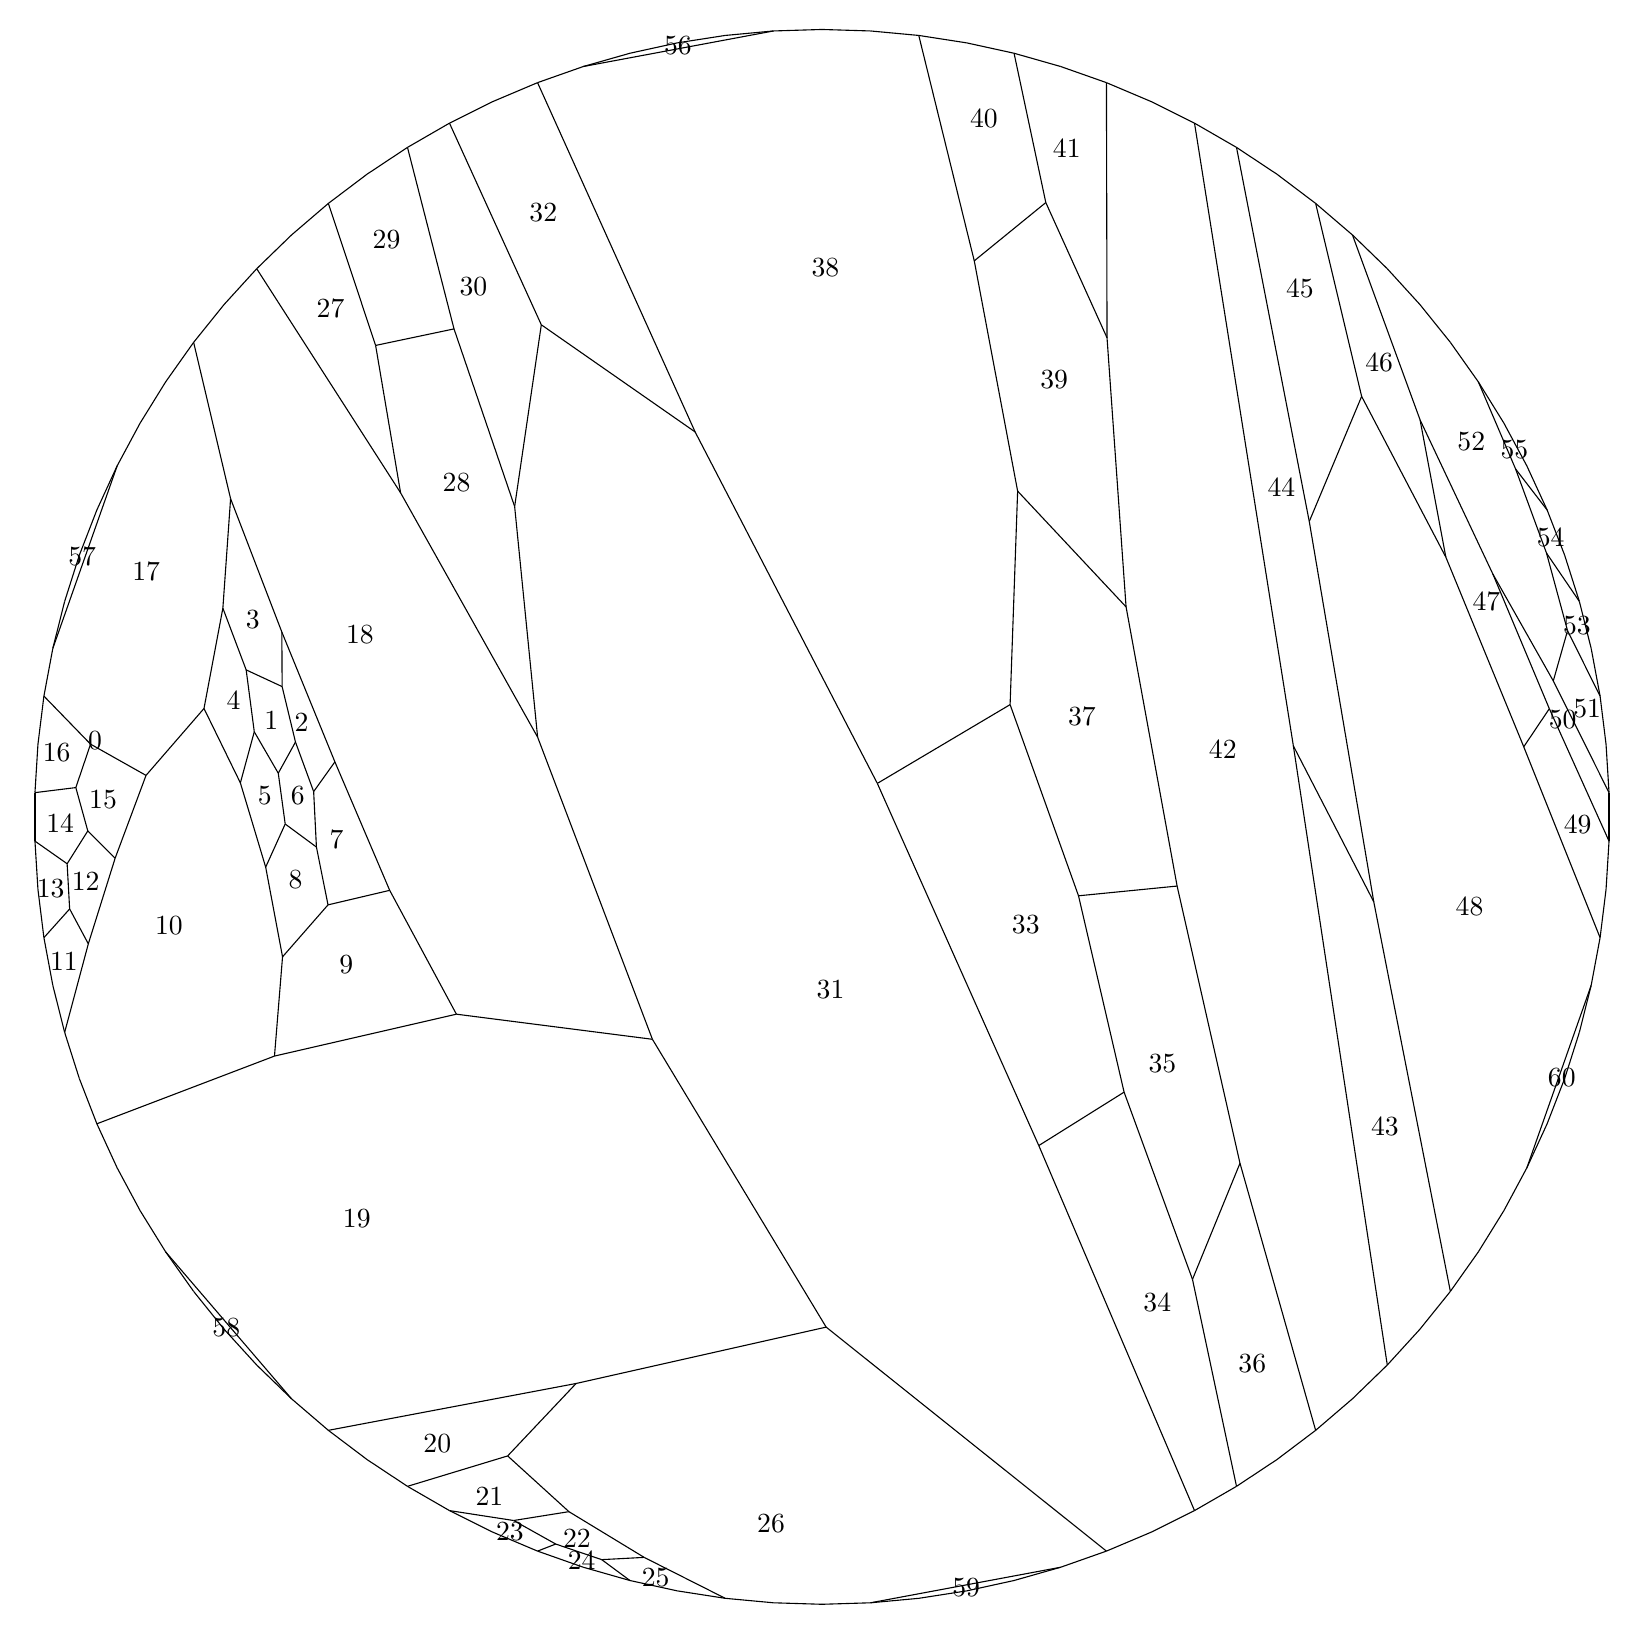
\begin{tikzpicture}[scale = 10, auto]
\coordinate (x0) at (-0.668668, 0.095025);
\coordinate (x1) at (-0.685642, 0.165465);
\coordinate (x2) at (-0.731296, 0.186654);
\coordinate (x3) at (-0.720998, 0.108076);
\coordinate (x4) at (-0.690517, 0.055461);
\coordinate (x5) at (-0.645580, 0.032069);
\coordinate (x6) at (-0.618618, 0.069871);
\coordinate (x7) at (-0.685971, 0.234711);
\coordinate (x8) at (-0.751087, 0.404079);
\coordinate (x9) at (-0.760876, 0.265049);
\coordinate (x10) at (-0.784845, 0.137658);
\coordinate (x11) at (-0.738643, 0.043176);
\coordinate (x12) at (-0.706519, -0.063820);
\coordinate (x13) at (-0.681728, -0.009051);
\coordinate (x14) at (-0.642082, -0.038298);
\coordinate (x15) at (-0.627357, -0.111755);
\coordinate (x16) at (-0.549015, -0.093311);
\coordinate (x17) at (-0.685107, -0.177740);
\coordinate (x18) at (-0.695335, -0.303794);
\coordinate (x19) at (-0.464287, -0.250577);
\coordinate (x20) at (-0.858468, 0.052688);
\coordinate (x21) at (-0.897711, -0.052524);
\coordinate (x22) at (-0.931770, -0.161242);
\coordinate (x23) at (-0.961826, -0.273663);
\coordinate (x24) at (-0.943154, -0.332355);
\coordinate (x25) at (-0.920906, -0.389786);
\coordinate (x26) at (-0.955475, -0.116925);
\coordinate (x27) at (-0.988165, -0.153392);
\coordinate (x28) at (-0.976848, -0.213933);
\coordinate (x29) at (-0.932421, -0.017849);
\coordinate (x30) at (-0.958660, -0.059532);
\coordinate (x31) at (-0.999526, -0.030795);
\coordinate (x32) at (-0.995734, -0.092268);
\coordinate (x33) at (-0.947632, 0.037202);
\coordinate (x34) at (-0.999526, 0.030795);
\coordinate (x35) at (-0.928921, 0.092359);
\coordinate (x36) at (-0.988165, 0.153392);
\coordinate (x37) at (-0.995734, 0.092268);
\coordinate (x38) at (-0.798017, 0.602635);
\coordinate (x39) at (-0.833602, 0.552365);
\coordinate (x40) at (-0.866025, 0.500000);
\coordinate (x41) at (-0.895163, 0.445738);
\coordinate (x42) at (-0.976848, 0.213933);
\coordinate (x43) at (-0.215374, -0.282460);
\coordinate (x44) at (-0.361140, 0.101243);
\coordinate (x45) at (-0.535184, 0.411565);
\coordinate (x46) at (-0.717912, 0.696134);
\coordinate (x47) at (-0.759405, 0.650618);
\coordinate (x48) at (-0.895163, -0.445738);
\coordinate (x49) at (-0.866025, -0.500000);
\coordinate (x50) at (-0.833602, -0.552365);
\coordinate (x51) at (-0.673696, -0.739009);
\coordinate (x52) at (-0.626924, -0.779081);
\coordinate (x53) at (-0.312288, -0.719588);
\coordinate (x54) at (0.005287, -0.647988);
\coordinate (x55) at (-0.577774, -0.816197);
\coordinate (x56) at (-0.526432, -0.850217);
\coordinate (x57) at (-0.399205, -0.811581);
\coordinate (x58) at (-0.473094, -0.881012);
\coordinate (x59) at (-0.391582, -0.893607);
\coordinate (x60) at (-0.321374, -0.882366);
\coordinate (x61) at (-0.338158, -0.923487);
\coordinate (x62) at (-0.279761, -0.943295);
\coordinate (x63) at (-0.225808, -0.940452);
\coordinate (x64) at (-0.417960, -0.908465);
\coordinate (x65) at (-0.361242, -0.932472);
\coordinate (x66) at (-0.303153, -0.952942);
\coordinate (x67) at (-0.243914, -0.969797);
\coordinate (x68) at (-0.183750, -0.982973);
\coordinate (x69) at (-0.122888, -0.992421);
\coordinate (x70) at (-0.061561, -0.998103);
\coordinate (x71) at (-0.000000, -1.000000);
\coordinate (x72) at (0.061561, -0.998103);
\coordinate (x73) at (0.303153, -0.952942);
\coordinate (x74) at (0.361242, -0.932472);
\coordinate (x75) at (-0.566888, 0.598741);
\coordinate (x76) at (-0.626924, 0.779081);
\coordinate (x77) at (-0.673696, 0.739009);
\coordinate (x78) at (-0.390331, 0.394090);
\coordinate (x79) at (-0.467326, 0.619728);
\coordinate (x80) at (-0.526432, 0.850217);
\coordinate (x81) at (-0.577774, 0.816197);
\coordinate (x82) at (-0.356467, 0.624952);
\coordinate (x83) at (-0.473094, 0.881012);
\coordinate (x84) at (0.417960, -0.908465);
\coordinate (x85) at (0.473094, -0.881012);
\coordinate (x86) at (0.275335, -0.417427);
\coordinate (x87) at (0.070285, 0.042522);
\coordinate (x88) at (-0.161112, 0.488847);
\coordinate (x89) at (-0.361242, 0.932472);
\coordinate (x90) at (-0.417960, 0.908465);
\coordinate (x91) at (0.383668, -0.349580);
\coordinate (x92) at (0.325770, -0.100235);
\coordinate (x93) at (0.238884, 0.142552);
\coordinate (x94) at (0.526432, -0.850217);
\coordinate (x95) at (0.470500, -0.587325);
\coordinate (x96) at (0.530838, -0.439900);
\coordinate (x97) at (0.450990, -0.087865);
\coordinate (x98) at (0.577774, -0.816197);
\coordinate (x99) at (0.626924, -0.779081);
\coordinate (x100) at (0.386167, 0.266693);
\coordinate (x101) at (0.248462, 0.413706);
\coordinate (x102) at (0.193374, 0.706155);
\coordinate (x103) at (0.122888, 0.992421);
\coordinate (x104) at (0.061561, 0.998103);
\coordinate (x105) at (0.000000, 1.000000);
\coordinate (x106) at (-0.061561, 0.998103);
\coordinate (x107) at (-0.303153, 0.952942);
\coordinate (x108) at (0.361979, 0.608454);
\coordinate (x109) at (0.284243, 0.780174);
\coordinate (x110) at (0.243914, 0.969797);
\coordinate (x111) at (0.183750, 0.982973);
\coordinate (x112) at (0.361242, 0.932472);
\coordinate (x113) at (0.303153, 0.952942);
\coordinate (x114) at (0.673696, -0.739009);
\coordinate (x115) at (0.717912, -0.696134);
\coordinate (x116) at (0.598640, 0.090154);
\coordinate (x117) at (0.473094, 0.881012);
\coordinate (x118) at (0.417960, 0.908465);
\coordinate (x119) at (0.759405, -0.650618);
\coordinate (x120) at (0.798017, -0.602635);
\coordinate (x121) at (0.700737, -0.107865);
\coordinate (x122) at (0.618822, 0.375172);
\coordinate (x123) at (0.526432, 0.850217);
\coordinate (x124) at (0.685341, 0.533981);
\coordinate (x125) at (0.626924, 0.779081);
\coordinate (x126) at (0.577774, 0.816197);
\coordinate (x127) at (0.792281, 0.329848);
\coordinate (x128) at (0.759556, 0.504203);
\coordinate (x129) at (0.673696, 0.739009);
\coordinate (x130) at (0.891217, 0.088999);
\coordinate (x131) at (0.923710, 0.137376);
\coordinate (x132) at (0.851999, 0.308357);
\coordinate (x133) at (0.833602, -0.552365);
\coordinate (x134) at (0.866025, -0.500000);
\coordinate (x135) at (0.895163, -0.445738);
\coordinate (x136) at (0.976848, -0.213933);
\coordinate (x137) at (0.988165, -0.153392);
\coordinate (x138) at (0.995734, -0.092268);
\coordinate (x139) at (0.999526, -0.030795);
\coordinate (x140) at (0.999526, 0.030795);
\coordinate (x141) at (0.928746, 0.172687);
\coordinate (x142) at (0.995734, 0.092268);
\coordinate (x143) at (0.988165, 0.153392);
\coordinate (x144) at (0.946836, 0.236487);
\coordinate (x145) at (0.920118, 0.334975);
\coordinate (x146) at (0.880850, 0.441851);
\coordinate (x147) at (0.833602, 0.552365);
\coordinate (x148) at (0.798017, 0.602635);
\coordinate (x149) at (0.759405, 0.650618);
\coordinate (x150) at (0.717912, 0.696134);
\coordinate (x151) at (0.976848, 0.213933);
\coordinate (x152) at (0.961826, 0.273663);
\coordinate (x153) at (0.943154, 0.332355);
\coordinate (x154) at (0.920906, 0.389786);
\coordinate (x155) at (0.895163, 0.445738);
\coordinate (x156) at (0.866025, 0.500000);
\coordinate (x157) at (-0.122888, 0.992421);
\coordinate (x158) at (-0.183750, 0.982973);
\coordinate (x159) at (-0.243914, 0.969797);
\coordinate (x160) at (-0.920906, 0.389786);
\coordinate (x161) at (-0.943154, 0.332355);
\coordinate (x162) at (-0.961826, 0.273663);
\coordinate (x163) at (-0.798017, -0.602635);
\coordinate (x164) at (-0.759405, -0.650618);
\coordinate (x165) at (-0.717912, -0.696134);
\coordinate (x166) at (0.122888, -0.992421);
\coordinate (x167) at (0.183750, -0.982973);
\coordinate (x168) at (0.243914, -0.969797);
\coordinate (x169) at (0.920906, -0.389786);
\coordinate (x170) at (0.943154, -0.332355);
\coordinate (x171) at (0.961826, -0.273663);
\draw (-0.668668, 0.095025) -- (-0.685642, 0.165465);
\draw (-0.685642, 0.165465) -- (-0.731296, 0.186654);
\draw (-0.731296, 0.186654) -- (-0.720998, 0.108076);
\draw (-0.720998, 0.108076) -- (-0.690517, 0.055461);
\draw (-0.690517, 0.055461) -- (-0.668668, 0.095025);
\draw (-0.668668, 0.095025) -- (-0.645580, 0.032069);
\draw (-0.645580, 0.032069) -- (-0.618618, 0.069871);
\draw (-0.618618, 0.069871) -- (-0.685971, 0.234711);
\draw (-0.685971, 0.234711) -- (-0.685642, 0.165465);
\draw (-0.685971, 0.234711) -- (-0.751087, 0.404079);
\draw (-0.751087, 0.404079) -- (-0.760876, 0.265049);
\draw (-0.760876, 0.265049) -- (-0.731296, 0.186654);
\draw (-0.760876, 0.265049) -- (-0.784845, 0.137658);
\draw (-0.784845, 0.137658) -- (-0.738643, 0.043176);
\draw (-0.738643, 0.043176) -- (-0.720998, 0.108076);
\draw (-0.738643, 0.043176) -- (-0.706519, -0.063820);
\draw (-0.706519, -0.063820) -- (-0.681728, -0.009051);
\draw (-0.681728, -0.009051) -- (-0.690517, 0.055461);
\draw (-0.681728, -0.009051) -- (-0.642082, -0.038298);
\draw (-0.642082, -0.038298) -- (-0.645580, 0.032069);
\draw (-0.642082, -0.038298) -- (-0.627357, -0.111755);
\draw (-0.627357, -0.111755) -- (-0.549015, -0.093311);
\draw (-0.549015, -0.093311) -- (-0.618618, 0.069871);
\draw (-0.706519, -0.063820) -- (-0.685107, -0.177740);
\draw (-0.685107, -0.177740) -- (-0.627357, -0.111755);
\draw (-0.685107, -0.177740) -- (-0.695335, -0.303794);
\draw (-0.695335, -0.303794) -- (-0.464287, -0.250577);
\draw (-0.464287, -0.250577) -- (-0.549015, -0.093311);
\draw (-0.784845, 0.137658) -- (-0.858468, 0.052688);
\draw (-0.858468, 0.052688) -- (-0.897711, -0.052524);
\draw (-0.897711, -0.052524) -- (-0.931770, -0.161242);
\draw (-0.931770, -0.161242) -- (-0.961826, -0.273663);
\draw (-0.961826, -0.273663) -- (-0.943154, -0.332355);
\draw (-0.943154, -0.332355) -- (-0.920906, -0.389786);
\draw (-0.920906, -0.389786) -- (-0.695335, -0.303794);
\draw (-0.931770, -0.161242) -- (-0.955475, -0.116925);
\draw (-0.955475, -0.116925) -- (-0.988165, -0.153392);
\draw (-0.988165, -0.153392) -- (-0.976848, -0.213933);
\draw (-0.976848, -0.213933) -- (-0.961826, -0.273663);
\draw (-0.897711, -0.052524) -- (-0.932421, -0.017849);
\draw (-0.932421, -0.017849) -- (-0.958660, -0.059532);
\draw (-0.958660, -0.059532) -- (-0.955475, -0.116925);
\draw (-0.958660, -0.059532) -- (-0.999526, -0.030795);
\draw (-0.999526, -0.030795) -- (-0.995734, -0.092268);
\draw (-0.995734, -0.092268) -- (-0.988165, -0.153392);
\draw (-0.932421, -0.017849) -- (-0.947632, 0.037202);
\draw (-0.947632, 0.037202) -- (-0.999526, 0.030795);
\draw (-0.999526, 0.030795) -- (-0.999526, -0.030795);
\draw (-0.858468, 0.052688) -- (-0.928921, 0.092359);
\draw (-0.928921, 0.092359) -- (-0.947632, 0.037202);
\draw (-0.928921, 0.092359) -- (-0.988165, 0.153392);
\draw (-0.988165, 0.153392) -- (-0.995734, 0.092268);
\draw (-0.995734, 0.092268) -- (-0.999526, 0.030795);
\draw (-0.751087, 0.404079) -- (-0.798017, 0.602635);
\draw (-0.798017, 0.602635) -- (-0.833602, 0.552365);
\draw (-0.833602, 0.552365) -- (-0.866025, 0.500000);
\draw (-0.866025, 0.500000) -- (-0.895163, 0.445738);
\draw (-0.895163, 0.445738) -- (-0.976848, 0.213933);
\draw (-0.976848, 0.213933) -- (-0.988165, 0.153392);
\draw (-0.464287, -0.250577) -- (-0.215374, -0.282460);
\draw (-0.215374, -0.282460) -- (-0.361140, 0.101243);
\draw (-0.361140, 0.101243) -- (-0.535184, 0.411565);
\draw (-0.535184, 0.411565) -- (-0.717912, 0.696134);
\draw (-0.717912, 0.696134) -- (-0.759405, 0.650618);
\draw (-0.759405, 0.650618) -- (-0.798017, 0.602635);
\draw (-0.920906, -0.389786) -- (-0.895163, -0.445738);
\draw (-0.895163, -0.445738) -- (-0.866025, -0.500000);
\draw (-0.866025, -0.500000) -- (-0.833602, -0.552365);
\draw (-0.833602, -0.552365) -- (-0.673696, -0.739009);
\draw (-0.673696, -0.739009) -- (-0.626924, -0.779081);
\draw (-0.626924, -0.779081) -- (-0.312288, -0.719588);
\draw (-0.312288, -0.719588) -- (0.005287, -0.647988);
\draw (0.005287, -0.647988) -- (-0.215374, -0.282460);
\draw (-0.626924, -0.779081) -- (-0.577774, -0.816197);
\draw (-0.577774, -0.816197) -- (-0.526432, -0.850217);
\draw (-0.526432, -0.850217) -- (-0.399205, -0.811581);
\draw (-0.399205, -0.811581) -- (-0.312288, -0.719588);
\draw (-0.526432, -0.850217) -- (-0.473094, -0.881012);
\draw (-0.473094, -0.881012) -- (-0.391582, -0.893607);
\draw (-0.391582, -0.893607) -- (-0.321374, -0.882366);
\draw (-0.321374, -0.882366) -- (-0.399205, -0.811581);
\draw (-0.391582, -0.893607) -- (-0.338158, -0.923487);
\draw (-0.338158, -0.923487) -- (-0.279761, -0.943295);
\draw (-0.279761, -0.943295) -- (-0.225808, -0.940452);
\draw (-0.225808, -0.940452) -- (-0.321374, -0.882366);
\draw (-0.473094, -0.881012) -- (-0.417960, -0.908465);
\draw (-0.417960, -0.908465) -- (-0.361242, -0.932472);
\draw (-0.361242, -0.932472) -- (-0.338158, -0.923487);
\draw (-0.361242, -0.932472) -- (-0.303153, -0.952942);
\draw (-0.303153, -0.952942) -- (-0.243914, -0.969797);
\draw (-0.243914, -0.969797) -- (-0.279761, -0.943295);
\draw (-0.243914, -0.969797) -- (-0.183750, -0.982973);
\draw (-0.183750, -0.982973) -- (-0.122888, -0.992421);
\draw (-0.122888, -0.992421) -- (-0.225808, -0.940452);
\draw (-0.122888, -0.992421) -- (-0.061561, -0.998103);
\draw (-0.061561, -0.998103) -- (-0.000000, -1.000000);
\draw (-0.000000, -1.000000) -- (0.061561, -0.998103);
\draw (0.061561, -0.998103) -- (0.303153, -0.952942);
\draw (0.303153, -0.952942) -- (0.361242, -0.932472);
\draw (0.361242, -0.932472) -- (0.005287, -0.647988);
\draw (-0.535184, 0.411565) -- (-0.566888, 0.598741);
\draw (-0.566888, 0.598741) -- (-0.626924, 0.779081);
\draw (-0.626924, 0.779081) -- (-0.673696, 0.739009);
\draw (-0.673696, 0.739009) -- (-0.717912, 0.696134);
\draw (-0.361140, 0.101243) -- (-0.390331, 0.394090);
\draw (-0.390331, 0.394090) -- (-0.467326, 0.619728);
\draw (-0.467326, 0.619728) -- (-0.566888, 0.598741);
\draw (-0.467326, 0.619728) -- (-0.526432, 0.850217);
\draw (-0.526432, 0.850217) -- (-0.577774, 0.816197);
\draw (-0.577774, 0.816197) -- (-0.626924, 0.779081);
\draw (-0.390331, 0.394090) -- (-0.356467, 0.624952);
\draw (-0.356467, 0.624952) -- (-0.473094, 0.881012);
\draw (-0.473094, 0.881012) -- (-0.526432, 0.850217);
\draw (0.361242, -0.932472) -- (0.417960, -0.908465);
\draw (0.417960, -0.908465) -- (0.473094, -0.881012);
\draw (0.473094, -0.881012) -- (0.275335, -0.417427);
\draw (0.275335, -0.417427) -- (0.070285, 0.042522);
\draw (0.070285, 0.042522) -- (-0.161112, 0.488847);
\draw (-0.161112, 0.488847) -- (-0.356467, 0.624952);
\draw (-0.161112, 0.488847) -- (-0.361242, 0.932472);
\draw (-0.361242, 0.932472) -- (-0.417960, 0.908465);
\draw (-0.417960, 0.908465) -- (-0.473094, 0.881012);
\draw (0.275335, -0.417427) -- (0.383668, -0.349580);
\draw (0.383668, -0.349580) -- (0.325770, -0.100235);
\draw (0.325770, -0.100235) -- (0.238884, 0.142552);
\draw (0.238884, 0.142552) -- (0.070285, 0.042522);
\draw (0.473094, -0.881012) -- (0.526432, -0.850217);
\draw (0.526432, -0.850217) -- (0.470500, -0.587325);
\draw (0.470500, -0.587325) -- (0.383668, -0.349580);
\draw (0.470500, -0.587325) -- (0.530838, -0.439900);
\draw (0.530838, -0.439900) -- (0.450990, -0.087865);
\draw (0.450990, -0.087865) -- (0.325770, -0.100235);
\draw (0.526432, -0.850217) -- (0.577774, -0.816197);
\draw (0.577774, -0.816197) -- (0.626924, -0.779081);
\draw (0.626924, -0.779081) -- (0.530838, -0.439900);
\draw (0.450990, -0.087865) -- (0.386167, 0.266693);
\draw (0.386167, 0.266693) -- (0.248462, 0.413706);
\draw (0.248462, 0.413706) -- (0.238884, 0.142552);
\draw (0.248462, 0.413706) -- (0.193374, 0.706155);
\draw (0.193374, 0.706155) -- (0.122888, 0.992421);
\draw (0.122888, 0.992421) -- (0.061561, 0.998103);
\draw (0.061561, 0.998103) -- (0.000000, 1.000000);
\draw (0.000000, 1.000000) -- (-0.061561, 0.998103);
\draw (-0.061561, 0.998103) -- (-0.303153, 0.952942);
\draw (-0.303153, 0.952942) -- (-0.361242, 0.932472);
\draw (0.386167, 0.266693) -- (0.361979, 0.608454);
\draw (0.361979, 0.608454) -- (0.284243, 0.780174);
\draw (0.284243, 0.780174) -- (0.193374, 0.706155);
\draw (0.284243, 0.780174) -- (0.243914, 0.969797);
\draw (0.243914, 0.969797) -- (0.183750, 0.982973);
\draw (0.183750, 0.982973) -- (0.122888, 0.992421);
\draw (0.361979, 0.608454) -- (0.361242, 0.932472);
\draw (0.361242, 0.932472) -- (0.303153, 0.952942);
\draw (0.303153, 0.952942) -- (0.243914, 0.969797);
\draw (0.626924, -0.779081) -- (0.673696, -0.739009);
\draw (0.673696, -0.739009) -- (0.717912, -0.696134);
\draw (0.717912, -0.696134) -- (0.598640, 0.090154);
\draw (0.598640, 0.090154) -- (0.473094, 0.881012);
\draw (0.473094, 0.881012) -- (0.417960, 0.908465);
\draw (0.417960, 0.908465) -- (0.361242, 0.932472);
\draw (0.717912, -0.696134) -- (0.759405, -0.650618);
\draw (0.759405, -0.650618) -- (0.798017, -0.602635);
\draw (0.798017, -0.602635) -- (0.700737, -0.107865);
\draw (0.700737, -0.107865) -- (0.598640, 0.090154);
\draw (0.700737, -0.107865) -- (0.618822, 0.375172);
\draw (0.618822, 0.375172) -- (0.526432, 0.850217);
\draw (0.526432, 0.850217) -- (0.473094, 0.881012);
\draw (0.618822, 0.375172) -- (0.685341, 0.533981);
\draw (0.685341, 0.533981) -- (0.626924, 0.779081);
\draw (0.626924, 0.779081) -- (0.577774, 0.816197);
\draw (0.577774, 0.816197) -- (0.526432, 0.850217);
\draw (0.685341, 0.533981) -- (0.792281, 0.329848);
\draw (0.792281, 0.329848) -- (0.759556, 0.504203);
\draw (0.759556, 0.504203) -- (0.673696, 0.739009);
\draw (0.673696, 0.739009) -- (0.626924, 0.779081);
\draw (0.792281, 0.329848) -- (0.891217, 0.088999);
\draw (0.891217, 0.088999) -- (0.923710, 0.137376);
\draw (0.923710, 0.137376) -- (0.851999, 0.308357);
\draw (0.851999, 0.308357) -- (0.759556, 0.504203);
\draw (0.798017, -0.602635) -- (0.833602, -0.552365);
\draw (0.833602, -0.552365) -- (0.866025, -0.500000);
\draw (0.866025, -0.500000) -- (0.895163, -0.445738);
\draw (0.895163, -0.445738) -- (0.976848, -0.213933);
\draw (0.976848, -0.213933) -- (0.988165, -0.153392);
\draw (0.988165, -0.153392) -- (0.891217, 0.088999);
\draw (0.988165, -0.153392) -- (0.995734, -0.092268);
\draw (0.995734, -0.092268) -- (0.999526, -0.030795);
\draw (0.999526, -0.030795) -- (0.923710, 0.137376);
\draw (0.999526, -0.030795) -- (0.999526, 0.030795);
\draw (0.999526, 0.030795) -- (0.928746, 0.172687);
\draw (0.928746, 0.172687) -- (0.851999, 0.308357);
\draw (0.999526, 0.030795) -- (0.995734, 0.092268);
\draw (0.995734, 0.092268) -- (0.988165, 0.153392);
\draw (0.988165, 0.153392) -- (0.946836, 0.236487);
\draw (0.946836, 0.236487) -- (0.928746, 0.172687);
\draw (0.946836, 0.236487) -- (0.920118, 0.334975);
\draw (0.920118, 0.334975) -- (0.880850, 0.441851);
\draw (0.880850, 0.441851) -- (0.833602, 0.552365);
\draw (0.833602, 0.552365) -- (0.798017, 0.602635);
\draw (0.798017, 0.602635) -- (0.759405, 0.650618);
\draw (0.759405, 0.650618) -- (0.717912, 0.696134);
\draw (0.717912, 0.696134) -- (0.673696, 0.739009);
\draw (0.988165, 0.153392) -- (0.976848, 0.213933);
\draw (0.976848, 0.213933) -- (0.961826, 0.273663);
\draw (0.961826, 0.273663) -- (0.920118, 0.334975);
\draw (0.961826, 0.273663) -- (0.943154, 0.332355);
\draw (0.943154, 0.332355) -- (0.920906, 0.389786);
\draw (0.920906, 0.389786) -- (0.880850, 0.441851);
\draw (0.920906, 0.389786) -- (0.895163, 0.445738);
\draw (0.895163, 0.445738) -- (0.866025, 0.500000);
\draw (0.866025, 0.500000) -- (0.833602, 0.552365);
\draw (-0.061561, 0.998103) -- (-0.122888, 0.992421);
\draw (-0.122888, 0.992421) -- (-0.183750, 0.982973);
\draw (-0.183750, 0.982973) -- (-0.243914, 0.969797);
\draw (-0.243914, 0.969797) -- (-0.303153, 0.952942);
\draw (-0.895163, 0.445738) -- (-0.920906, 0.389786);
\draw (-0.920906, 0.389786) -- (-0.943154, 0.332355);
\draw (-0.943154, 0.332355) -- (-0.961826, 0.273663);
\draw (-0.961826, 0.273663) -- (-0.976848, 0.213933);
\draw (-0.833602, -0.552365) -- (-0.798017, -0.602635);
\draw (-0.798017, -0.602635) -- (-0.759405, -0.650618);
\draw (-0.759405, -0.650618) -- (-0.717912, -0.696134);
\draw (-0.717912, -0.696134) -- (-0.673696, -0.739009);
\draw (0.061561, -0.998103) -- (0.122888, -0.992421);
\draw (0.122888, -0.992421) -- (0.183750, -0.982973);
\draw (0.183750, -0.982973) -- (0.243914, -0.969797);
\draw (0.243914, -0.969797) -- (0.303153, -0.952942);
\draw (0.895163, -0.445738) -- (0.920906, -0.389786);
\draw (0.920906, -0.389786) -- (0.943154, -0.332355);
\draw (0.943154, -0.332355) -- (0.961826, -0.273663);
\draw (0.961826, -0.273663) -- (0.976848, -0.213933);
\node at (-0.923074, 0.096932) {0};
\node at (-0.699424, 0.122136) {1};
\node at (-0.660896, 0.119428) {2};
\node at (-0.722974, 0.251192) {3};
\node at (-0.747331, 0.148123) {4};
\node at (-0.707681, 0.026769) {5};
\node at (-0.665715, 0.027041) {6};
\node at (-0.616530, -0.028285) {7};
\node at (-0.668559, -0.080133) {8};
\node at (-0.604220, -0.187435) {9};
\node at (-0.829480, -0.138309) {10};
\node at (-0.962817, -0.183831) {11};
\node at (-0.935208, -0.081614) {12};
\node at (-0.979512, -0.090582) {13};
\node at (-0.967553, -0.008036) {14};
\node at (-0.913031, 0.022375) {15};
\node at (-0.971996, 0.081203) {16};
\node at (-0.858365, 0.310900) {17};
\node at (-0.586910, 0.231319) {18};
\node at (-0.590756, -0.510035) {19};
\node at (-0.488525, -0.795333) {20};
\node at (-0.422337, -0.863757) {21};
\node at (-0.311337, -0.916641) {22};
\node at (-0.396407, -0.907809) {23};
\node at (-0.305245, -0.944399) {24};
\node at (-0.211224, -0.965788) {25};
\node at (-0.064717, -0.897820) {26};
\node at (-0.624121, 0.644906) {27};
\node at (-0.464174, 0.425073) {28};
\node at (-0.553069, 0.732793) {29};
\node at (-0.442730, 0.674000) {30};
\node at (0.010798, -0.219834) {31};
\node at (-0.353975, 0.767150) {32};
\node at (0.258788, -0.136434) {33};
\node at (0.425806, -0.617112) {34};
\node at (0.432353, -0.312981) {35};
\node at (0.546494, -0.694544) {36};
\node at (0.330055, 0.126970) {37};
\node at (0.004399, 0.697075) {38};
\node at (0.294845, 0.555036) {39};
\node at (0.205634, 0.886304) {40};
\node at (0.310906, 0.848768) {41};
\node at (0.509040, 0.085933) {42};
\node at (0.714942, -0.393420) {43};
\node at (0.583545, 0.417738) {44};
\node at (0.607059, 0.670930) {45};
\node at (0.707560, 0.577224) {46};
\node at (0.843752, 0.273756) {47};
\node at (0.822384, -0.113448) {48};
\node at (0.959670, -0.010016) {49};
\node at (0.940701, 0.123684) {50};
\node at (0.971802, 0.137126) {51};
\node at (0.824612, 0.476302) {52};
\node at (0.958759, 0.242490) {53};
\node at (0.925371, 0.354526) {54};
\node at (0.879309, 0.465948) {55};
\node at (-0.183053, 0.979247) {56};
\node at (-0.939579, 0.331095) {57};
\node at (-0.756526, -0.648152) {58};
\node at (0.183053, -0.979247) {59};
\node at (0.939579, -0.331095) {60};
\end{tikzpicture}
\caption{Graph}

\end{figure}
\end{document}

        \end{scope}
        \\
        \begin{scope}[scale=3, yshift=25]
          \coordinate (x0) at (0.606503, -0.203815);
\coordinate (x1) at (0.564996, -0.270265);
\coordinate (x2) at (0.540011, -0.344783);
\coordinate (x3) at (0.536642, -0.433914);
\coordinate (x4) at (0.548348, -0.525342);
\coordinate (x5) at (0.715196, -0.344188);
\coordinate (x6) at (0.752873, -0.100796);
\coordinate (x7) at (0.674083, -0.146762);
\coordinate (x8) at (0.550670, -0.226115);
\coordinate (x9) at (0.525551, -0.286272);
\coordinate (x10) at (0.638050, -0.131824);
\coordinate (x11) at (0.586196, -0.195596);
\coordinate (x12) at (0.552287, -0.264252);
\coordinate (x13) at (0.520471, -0.334052);
\coordinate (x14) at (0.502267, -0.415166);
\coordinate (x15) at (0.801620, 0.143300);
\coordinate (x16) at (0.692674, -0.070484);
\coordinate (x17) at (0.588716, -0.283231);
\coordinate (x18) at (0.487181, -0.497178);
\coordinate (x19) at (0.387853, -0.715827);
\coordinate (x20) at (0.222521, -0.974928);
\coordinate (x21) at (0.900969, -0.433884);
\coordinate (x22) at (0.900969, 0.433884);
\coordinate (x23) at (0.222521, 0.974928);
\coordinate (x24) at (-0.623490, 0.781831);
\coordinate (x25) at (-1.000000, 0.000000);
\coordinate (x26) at (-0.623490, -0.781831);
\draw (x0) -- (x1);
\draw (x1) -- (x2);
\draw (x2) -- (x3);
\draw (x3) -- (x4);
\draw (x4) -- (x5);
\draw (x5) -- (x6);
\draw (x6) -- (x7);
\draw (x7) -- (x0);
\draw (x0) -- (x8);
\draw (x8) -- (x9);
\draw (x9) -- (x2);
\draw (x7) -- (x10);
\draw (x10) -- (x11);
\draw (x11) -- (x8);
\draw (x11) -- (x12);
\draw (x12) -- (x13);
\draw (x13) -- (x9);
\draw (x13) -- (x14);
\draw (x14) -- (x3);
\draw (x6) -- (x15);
\draw (x15) -- (x16);
\draw (x16) -- (x10);
\draw (x16) -- (x17);
\draw (x17) -- (x12);
\draw (x17) -- (x18);
\draw (x18) -- (x14);
\draw (x18) -- (x19);
\draw (x19) -- (x4);
\draw (x19) -- (x20);
\draw (x20) -- (x21);
\draw (x21) -- (x5);
\draw (x21) -- (x22);
\draw (x22) -- (x15);
\draw (x22) -- (x23);
\draw (x23) -- (x24);
\draw (x24) -- (x25);
\draw (x25) -- (x26);
\draw (x26) -- (x20);
\node at (-0.000000, -0.000000) {0};
\node at (0.617332, -0.296233) {1};
\node at (0.557546, -0.266250) {2};
\node at (0.611100, -0.180822) {3};
\node at (0.547035, -0.261257) {4};
\node at (0.524989, -0.362837) {5};
\node at (0.711860, -0.061313) {6};
\node at (0.611584, -0.189077) {7};
\node at (0.530184, -0.358776) {8};
\node at (0.492458, -0.517485) {9};
\node at (0.554977, -0.598834) {10};
\node at (0.814325, -0.060337) {11};
\node at (0.187007, -0.089958) {12};

        \end{scope}
        \\
      };
    \end{tikzfigure}
  \end{proof}
\end{theorem}